%!TEX root = ../../thesis.tex
%!TEX enableSynctex = true
%*******************************************************************************
%*********************************** First Chapter *****************************
%*******************************************************************************

\definecolor{455nm}{RGB}{0,97,255}
\definecolor{488nm}{RGB}{0,247,255}
\definecolor{561nm}{RGB}{198,255,0}
\definecolor{647nm}{RGB}{255,0,0}
\definecolor{illustrator_red}{RGB}{226,7,25}
\definecolor{illustrator_green}{RGB}{0,150,64}

\ifpdf
    \graphicspath{{Chapters/design/Figs/Raster/}{Chapters/design/Figs/PDF/}{Chapters/design/Figs/}}
\else
    \graphicspath{{Chapters/design/Figs/Vector/}{Chapters/design/Figs/}}
\fi

% Chapter 3.	Microscope design
% 3.1	Design objectives	59
% 3.2	Optical design	59
% 3.3	Mechanical design	64
% 3.4	Assembly	67
% 3.5	Control	68
% 3.6	Orientation, Alignment and Calibration	73
% 3.7	Initial results	74
% 3.8	Design summary	81


\chapter{Light-sheet microscope design and considerations }\label{chapter:design}

% \epigraph{\emph{It doesn't have to be good, it just has to look good.}}%{--- Anonymous}
%Physical prciniples of the operation of a light-microscope.
%Capabilities limtiations.

This chapter introduces the instrument which was built and used during this thesis.
It was required that the system presented here facilitated a wide range of imaging challenges, with two specific %biological aims to be met.
imaging tasks to be performed.
The first %of which task required the system to
task was to image Zebrafish embryos (\SI{\sim500}{\micro\meter}), surrounded by a magnetic tweezer system, during the \SI{1}{}k~cell stage of embryo development (see Chapter~\ref{chapter:tweezers}); this was for the study of developmental mechanobiology.
The second required the imaging of live (SHSY5Y) mammalian cells (\SI{\sim50}{\micro\meter}) for viral particulate tracking; this was for the study of 3D-live-cell viral egress using SPT.\@
\pagebreak
\subsection*{Specification}\label{sec:specification}

To facilitate these biological aims the system has to address these specification key criteria:

\begin{enumerate}
    \item Fast volumetric imaging, 1 volume per second for the pixel range:\\\SI{2048x2048x100}{}\label{item:volumes}
    \item Multi-colour interlaced volumetric imaging  \label{item:colour}
    \item Capacity for multiple methods of sample mounting \label{item:mounting}
    \item Multiple imaging length scales, \gls{FOV} range :~\SIrange{200}{700}{\micro\meter} \label{item:scales}% magnifications
    \item Options for exotic illumination development through optional illumination paths to incorporate an \gls{SLM} \label{item:illumination}
    \item User-friendly and extensible software scheme in \gls{LabVIEW} \label{item:software}
\end{enumerate}

% \subsection{Embryonic imaging for Mechanobiology}
%
% For embryonic imaging using magnetic tweezers the system had to be designed with sufficient space
%
% \subsection{Cellular imaging for Viral Egress}
%
% To realise particle tracking within light sheet microscope improvements upon the previous system were considered and the entire microscope was to be rebuilt using a new design.
% Any optical development project comprises of a series of sub-systems, modules which can be built and designed so that the overall scale of the project is made more manageable.
% A microscope of this nature will have typically four aspects:
%
% \begin{itemize}
% 	\item Sample Holding
% 	\item Illumination
% 	\item Detection
% 	\item Image Acquisition
% \end{itemize}
%
% Though each section may somewhat affect the others key decisions and debugging can usually be localised to each.
% This section will discuss the new design, improvements upon the previous design and the current build state of the microscope for each of these components of the new system.

\section{Hardware}

The design presented here is an adaptation of a previous \gls{light-sheet} microscope, whose entire optical assembly was mounted on a set of rails rotated at \SI{45}{\degree}.
The upgrade and redesign of the system was made such that the illumination and detection paths of the new system could be extended so that liquid tuneable lenses could be mounted in the vertically to reduce gravity induced optical aberrations.

The new design presented in this thesis adapts a previous design.
For precise tracking of single virions, a more stabilised method of suspending the microscope objectives was needed as this minimises vibrational blur.
This was problematic in the previous design due to design using cantilevered detection optics away from the frame, causing general instability.
% suspension of objectives was needed.

\subsection{Mechanical design}

% \gls{illumination arm}
% \gls{detection arm}
% \gls{imaging board}
% \gls{illumination board}
% \gls{imaging optical rail}
% \gls{illumination board}
% \gls{imaging board}

The mechanical design of the \gls{light-sheet} microscope consists of two optical breadboards, mounted one above the other.
One for mounting the light sources (\gls{illumination board}) and the second (\gls{imaging board}) for the \glslink{illumination arm}{illumination} and \glslink{detection arm}{detection} arms.
The \gls{imaging board} was mounted vertically above the \gls{illumination board} on \SI{50.8}{\milli\metre} stabilising metal posts, which ensured the system was transportable as well as robust against vibrations.
A large rectangular section of material was removed from the \gls{imaging board} to allow the objective lenses to reach down to the samples inserted from below; too large of a gap would lead to excessive sag and vibrations in each arm, too small would impede access to the sample below the imaging board.
The objective lenses and detection objective actuator were mounted on rails at \SI{45}{\degree} to the \gls{imaging board}, the \glslink{illumination arm}{illumination} and \glslink{detection arm}{detection} arms.
These rails guided the objectives through the open section until the focal points of each objective (detection and illumination) met.
The filter wheel was placed on the \gls{imaging optical rail} before the camera and after a turning mirror on the \gls{detection arm}
% and auxiliary supports
so that the vibrations, due to
 % so that vibrations of
filter switching and the camera fan, would be mostly decoupled from the detection optics.
The camera was mounted at \SI{45}{\degree} on a \gls{3D} printed mount that corrected for the turning mirror on the \gls{imaging optical rail}.
Rotating the camera was necessary as it allowed the camera shutter and illumination beam to propagate concomitantly for slit-scanning, see later Chapter~\ref{chapter:dualslit}.

For the illumination path, a \SI{22.5}{\degree} mirror
(to the horizon, see \figurename~\ref{fig:soldiworks_top}~(d))
was used to deliver the laser illumination from the scanning optics into the illumination objective on the \gls{illumination arm}.
The additional mirror was needed so that the scanning optics could be mounted flat to the optical breadboard, making positioning and optical mounting simpler.
Using two mirrors also provided the sufficient degrees of freedom to align the axis of the scanning optics to the optical axis along the \gls{illumination arm}.
Finally, the light-sheet generating mirror of the scanning pair of was suspended off the edge of the breadboard for delivery of the  illumination from the bottom optical table, see \figurename\ref{fig:soldiworks_top}~(a).

% Mechanical design changes for more stable an extensible system than previous work.
% Large detection area for future upgrades on detection arm - Like my relaying
% Space below for exotic excitation and large complex biological chambers, see Tweezers Chjapter.

%The small reflection angles required by the SLM and long detection FLIM arm were incompatible with the LSFM system and a new mechanical design was necessary (Figure 7.2).


%Instead of positioning all the optical components in the 45o frame, only the detection path, the excitation objective and the tube lens were mounted at this angle.
%A mirror at 22.5o to horizontal reoriented excitation path vertically.
%Hence, a simpler frame was sufficient, consisting of two optical breadboards – one above the other.
%The dSLM optics and detection was mounted on the top level, while SLM and laser on the bottom level.
%A hole was cut in top breadboard so that the ‘V’ shaped arrangement of objectives was suspended below it.
%The sample translation stage was placed on the bottom breadboard and elevated to reach the imaging volume.
%The detection cage system included a 450 mirror which ensured that the long FLIM arm could be mounted horizontally above the top breadboard.

% Besides additional compatibility with upgrades, this design was more mechanically stable and had a large sample space for complex biological chambers.
% Moreover the tuneable lenses were positioned horizontally in a vertical cage system avoiding gravitational deformations and hence aberrations.

\subsubsection{Sample mounting}

%SPIM is notorious for sample mounting within the microscopy community, this is due to
Sample mounting using light-sheet microscopes can be challenging due to the need to place a secondary objective (for illumination) within close proximity to the detection objective.
The concept of the \gls{iSPIM}~\cite{wuInvertedSelectivePlane2011a} allows more freedom in terms of sample mounting as more of the image volume is accessible.
The \gls{imaging board} was mounted \SI{500}{\milli\meter} above the \gls{illumination board} so that an XYZ translator, with a large axial range, could be mounted.
This allowed for multiple potential sample mounting strategies below.
%This design point is one of the axioms of the new system, the focus of this report.

%The microscope system was designed using \SI{45}{\degree} \textbf{C}omputer \textbf{A}ided \textbf{D}esign so that two objectives would be mounted on \SI{45}{\degree} rails, allowing a detection and excitation objective to be lowered into a imaging space below.
%Each rail comprised of two \SI{16}{\milli\meter} to \SI{8}{\milli\meter} caging conversion mounts.
%The \SI{16}{\milli\meter} mounts were attached to the rail by two guides placed in parallel to ensure that the objectives were in the same plane and correct angle.
%The objectives were held on \SI{8}{\milli\meter} caging which attached to a thumb-screw mount holding each objective, so that they could both be very precisely lowered for fine adjustments.
%The \SI{8}{\milli\meter} caging also carried an aluminium cube suitable for dynamically lowering a beam splitter or mirror into the system so that issues on excitation could be diagnosed, as the diverted light would be the exact the image of the back aperture of the excitation objective.
%Each rail was then mounted on an optical breadboard, with a noise dampening core to limit vibrations.

%To allow the inverted objectives access to the samples the optical breadboard was cut with sufficient tolerance to allow them through but maintaining their stability; too large of a gap would cause sag in each arm, too small would impede access to the sample below.
%The hole was calculated using precision Solidworks, see Figure \ref{fig:solidworks_design_front}.
%This breadboard was then elevated to a height of \SI{50}{\centi\meter}, using $25mm$ diameter aluminium posts for stability and vibrational dampening.
%The posts were mounted on a secondary optical breadboard which supported excitation optical components.
%The secondary breadboard was implemented with the ambition that the entire microscope could be ``portable" as it did not have a permanent residence where it was being built.
%Hardware as well as a digitally controlled XYZ stage was placed on the bottom breadboard.

\paragraph{XYZ stage}

A \emph{Prior} Pro Scan \textit{HLD117} XY stage was mounted on top of a Motorized Linear Axis \textit{FB204E} Z stage.
The set was chosen as each component had integrated linear encoders, giving a suitable positional resolution (\SI{20}{\nano\meter} in \(xyz\));
speed \SI{300}{\milli\meter\per\second} in \(xy\) and \SI{15}{\milli\meter\per\second} in \(z\);
large travel range (\(\SI{120}{\milli\meter} \times \SI{72}{\milli\meter} \) in \(xy\) and \SI{38}{\milli\meter} in \(z\))% and versatility in terms of mounting onto the microscope and sample mountings and their ability for computer interfacing~\cite{Hu2014}.
Each component was also computer controllable, and an open-source \gls{LabVIEW} routine was developed and made freely available for this purpose~\cite{russellSpimcontroller2017}.
%
% \subsubsection{Comparison with old SPIM}
%
% The original SPIM design also used a dual inverted layout, but crucially, its detection and excitation arms were not as well seated.
% Each arm was held orthogonally to gravity, meaning each acted like a cantilever, bending unstably and unpredictably under its own weight.
% This moment meant that the system was less stable than the new design and very susceptible to vibrations, which add systematic noise that can not be corrected for.
% The old SPIM also lacked in that it did not have any motorised XYZ translation, this meant that is could not achieve large area imaging, high-throughput experiments nor could it facilitate single particle tracking in thick samples.
%\subsection{iSPIM Design}
%All demonstrations of the 4~pt correction were performed on an iSPIM (\emph{inverted Selective Plane Imaging Microscope}).
\begin{landscape}
  \begin{figure}
  \centering
  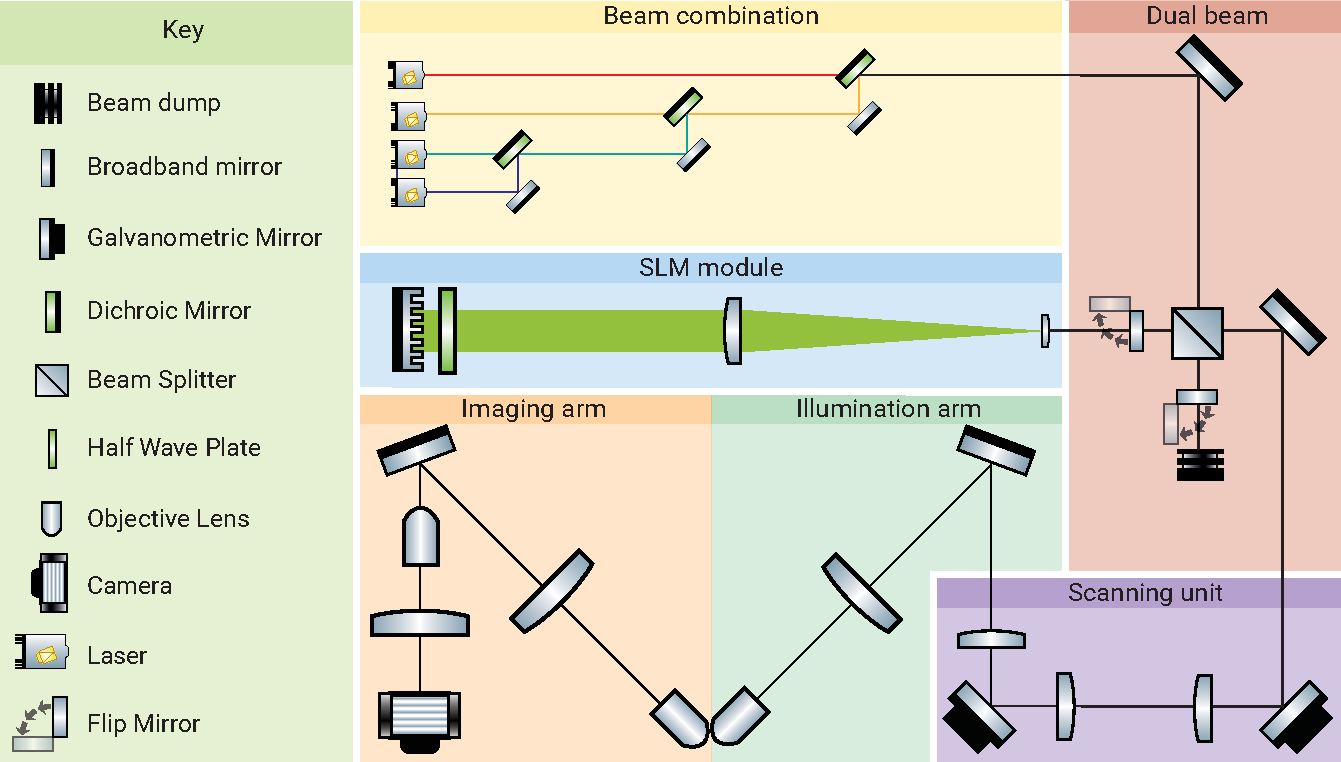
\includegraphics[width=\linewidth]{./optical_design_colour}
  \caption[Full optical design of new \gls{light-sheet} microscope]{
  Optical design of the light-sheet microscope. \textbf{Yellow:} Beam comination of the four laser lines using dichroic mirrors.
  \textbf{Red:} a beam splitter is used to create two beam arms which can be used together to create two parallel beams; one beam for single beam light-sheet; or one beam structured using the SLM (blue).
  \textbf{Blue:} Expansion optics for the optional SLM arm of the illumination system.
  \textbf{Purple:} A pair of scanning galvanometric mirrors are relayed onto each other and passed through a scan lens.
  \textbf{Green:} The illumination arm where the scanning beam is demagnified onto the sample.
  \textbf{Orange:} The high NA detection optics magnify the sample onto a second magnifying relay system and finally onto the camera.
  %Optical design of the new SPIM microscope.
  %Straight black lines represent mirrors; arrowed lines represent lenses; coloured lines represent laser light.
  }\label{fig:optical_design_colour}
  \end{figure}
\end{landscape}

% A (\emph{Coherent Obis 561nm}) laser was used as the beam source.
% A pair of galvanometric mirrors (\emph{Cambridge Technology}) were used to produce 2D beam steering via an image relay, this approach is well established in scanning microscopy and is known to introduce ordinarily negligible field curvature.
% A telecentric scan lens (\emph{A1 Scan Lens} from Nikon) was used to convert beam angle to beam position; %\footnote{The exact make and model will not be mentioned the manufacturers do not wish for characterisation data to be published without their express permission}
% within the observation volume this acts to keep the sweeping beam parallel for a homogenous illumination and background.
% A (\emph{10x 0.3 NA Nikon}) water dipping objective was used for excitation and mounted at right angles to a (\emph{25x 1.1 NA}) Nikon LWD water immersion objective.
% The fluorescence collected by the detection objective is then imaged onto a Hamamatsu sCMOS Orca Flash 4.
% A piezo scanner (\emph{Physik Instrumente P-726 PIFOC high-load objective scanner}) was used to manually move the detection objective to match the detection focal plane to the excitation plane.
\subsection{Optical design}

\subsection{Objective lenses}

%\nomenclature[z-WD]{WD}{WD of View}

A (\emph{\(10\times 0.3 \gls{NA}\)}) Nikon water-dipping objective was used for illumination and mounted at right angles to a (\emph{\(25\times1.1 \gls{NA}\)}) Nikon LWD water immersion objective.
The water dipping objective used here has a \SI{3.5}{\milli\meter} WD and narrow physical profile; meaning that when matched with the bulkier high NA detection objective
there would be mechanical overlap if collimated light was coupled into the illumination lenses.
Instead, the illumination tube lens supplied slightly diverging light to the back aperture of the illumination objective, which was found to efficiently resolve the challenge of separating the detection and illumination objective lenses.
%there was a slight mechanically interference, which was corrected for using the tube lens to adjust the working distance.
%, once their positioned with their foci were co-aligned.
Very few objective pairs maximise detection and illumination \gls{NA} whilst being water dipping and compatible, and a solution the solution Chapter~\ref{chapter:chamber} was found to be effective for imaging.
A piezo scanner (Physik Instrumente~\emph{P-726 PIFOC high-load objective scanner}) was used to manually move the detection objective to match the detection focal plane to the illumination plane.

\subsection{Illumination}

Four %typical
laser sources were chosen to allow good specificity across the visible spectrum as well  as for multi-colour imaging.
%, future-proofing and overall versatility in the microscope.
Wavelengths \textcolor{455nm}{\SI{455}{\nano\meter}},  \textcolor{488nm}{\SI{488}{\nano\meter}},  \textcolor{561nm}{\SI{561}{\nano\meter}} and \textcolor{647nm}{\SI{647}{\nano\meter}} were chosen to excite typical fluorescent exciters of commercially available fluorophores in the visible range.
The output power of the lasers (\SI{100}{\milli\watt}) was sufficient for good contrast images in SPIM.\@
\footnote{SPIM is within the single sun power regime} %TODO expand
%A beam quality $M^2$ nearing 1 is good, with $M^2 = 1$ being a theoretical ideal.
%Over the range of a metre the lasers will diverge by \SI{1.2}{\milli\meter}, though this would double the beam diameter the sizes are appreciably small that it will have very little effect when corrected for through later optics.
%See Table \ref{table:laser} for a detailed specification.
The beams were combined %into an overlapping beam using a set of standard dielectric mirrors and dichroic mirrors.
%Using two mirrors per beam allowed the degrees of freedom to accurately combine the beams in free space.
using dichroic mirrors % were chosen to ensure the each laser line propagated freely when approaching from behind the mirror but the correct colour laser was reflected appropriately; they were placed in the order e02 (dielectric as the first laser does not combine with any others)
(Chroma~\emph{zt594rdc, zt514rdc}~and~\emph{zt458rdc}) and broadband dielectric mirrors,
the illumination setup is illustrated in \figurename~\ref{fig:optical_design_colour}.
%See \figurename~\ref{fig:optical_design_colour}.

An alternative to using independent laser lines is using a white light laser source with chromatic notch filters. %and using the dichroic mirrors as long pass filters whilst using other filters to create the short pass.
To modulate the power for each channel would require fast intensity modulation potentially using an \gls{AOTF}.
%If this were the case then the power of each individual laser line would be dependent on the other laser lines.
%To then circumvent this an intensity modulator such as an
% would be needed as well.
%The former solution is more economical and more predictable.
White light sources (e.g. Fianium \emph{SC390} supercontinuum lasers) are expensive; do not produce homogeneous emissions;
%as well as the overall solution being more costly.
are more costly as well as the class 4 laser beam being intrinsically more hazardous than the class 3b diode laser in this design.
%, each colour may have been wholly variant in terms of quality for instance.

\subsection{Light-sheet generation}

For generation of the \gls{light-sheet} a \glslink{galvanometric scanning mirrors}{galvanometric scanning mirror} (\emph{Cambridge Technology}) was placed behind a \gls{telecentric} scan lens.
The \gls{telecentric} lens converts incident angle to emitted position such that a scanning mirror placed on-axis one focal distance behind the lens will produce a paraxial sweeping beam.
The \gls{light-sheet} generating scanning mirror was conjugated using a pair of matched lenses, in a \gls{4f} configuration, on a second scanning mirror.
The second mirror was mounted at \SI{90}{\degree} to the light-sheet generating mirror to allow the sheet be displaced move axially with respect to the imaging lens.
This allowed for fast volumetric imaging as well as correction for distortions caused by the scanning optics, discussed further in Chapter~\ref{chapter:homography}.
\figurename~\ref{fig:soldiworks_top} presents a schematic of light sheet generation.

% To generate a virtual light sheet a telecentric (sometimes called an f theta lens) is used to translate scanning mirror angle into a laser position shift creating a light sheet from a static laser beam.
% This lens couples with the tube lens to partially fill the back aperture of the objective so that a suitably thin light sheet is produced, with an ideal field of view tuned to compensate for the Gaussian profile of laser light.

% \subsubsection{Cage System}
%
% The light sheet generation components were all housed in cage system optomechanics as opposed to the free space optics of the bottom breadboard.
% The cage system was used as it projects the sensitive galvanometer mirrors as well as make lens alignment easier as the cage system \textit{should} remove off axis by virtue.
\clearpage
\begin{figure}
    \centering
    \begin{subfigure}[b]{\textwidth}
        \centering
        \includegraphics{spim_cad_side}
        \caption{\gls{CAD} model of \gls{light-sheet} microscope from the side, gravity is down}
        \label{fig:solidworks_design_front}
    \end{subfigure}
\end{figure}
\clearpage
\begin{figure}
    \ContinuedFloat
    \begin{subfigure}[b]{\textwidth}
        \centering
        \includegraphics{spim_cad_top}
        \caption{\gls{CAD} model of \gls{light-sheet} microscope from the top, gravity is going through the page}
        \label{fig:soldiworks_top}
    \end{subfigure}   % \ContinuedFloat
\end{figure}
\begin{figure}
        \ContinuedFloat
    \caption[\gls{CAD} three dimensional representation of the \SI{45}{\degree} inverted geometry imaging breadboard]{
    \gls{CAD} three dimensional representation of the \SI{45}{\degree} inverted geometry imaging breadboard.
    Sample access is allowed from beneath whilst still creating a fully orthogonal detection and illumination system.
    The coordinate system was chosen with the imaging axis being coaxial with the the axially direction (\(z\)) in the imaging direction, and right-handed with the \(x\) direction into the page and \(y\) in the direction of propagation of the illumination.\\
    \textcolor{illustrator_green}{\textbf{↑IL}}: Illumination comes from below on the right of the diagram.
    \textcolor{illustrator_green}{\textbf{SM1}}: Scan mirror, generates the \gls{light-sheet}.
    \textcolor{illustrator_green}{\textbf{SMR}}: Scan mirror relay, optically relays image of \textcolor{illustrator_green}{\textbf{SM1}} onto \textcolor{illustrator_green}{\textbf{SM2}}.
    \textcolor{illustrator_green}{\textbf{SM2}}: Scan mirror, moves the \gls{light-sheet} axially.
    \textcolor{illustrator_green}{\textbf{SL}}: Scan lens, keeps the \gls{light-sheet} par-axial at the specimen plane.
    \textcolor{illustrator_green}{\textbf{TM}}: Turning mirror (\SI{22.5}{\degree}), redirects the \gls{light-sheet} into \gls{illumination arm}.
    \textcolor{illustrator_green}{\textbf{TL}}: Tube lens (\emph{ITL200}), focuses collimated illumination light into the back aperture of the illumination objective \textcolor{illustrator_green}{\textbf{OBJ}}. Objective lens, for illumination.\\
    \textcolor{illustrator_red}{\textbf{OBJ}}: Objective lens, for imaging.
    \textcolor{illustrator_red}{\textbf{TL}}: Tube lens (\emph{ITL200}), images specimen plane to an image plane
    \textcolor{illustrator_red}{\textbf{TM}}: Turning mirror (\SI{22.5}{\degree}), redirects the emitted light into \gls{imaging optical rail}.
    \textcolor{illustrator_red}{\textbf{OBJ-R}}: Objective relay, on a turret for choosing multiple magnifications.
    \textcolor{illustrator_red}{\textbf{FW}}: Filter wheel, for rejecting the non-fluorescent signal.
    \textcolor{illustrator_red}{\textbf{TL-R}}: Tube lens relay, for imaging the relayed image plane onto the camera (CAM).
    \textcolor{illustrator_red}{\textbf{CAM}}: Camera (sCMOS, Hamamatsu Orca Flash 4 v2.0), for detection of the fluorescent signal.
    }\label{fig:soldiworks_top}

    % \textcolor{illustrator_red}{OBJ}. {OBJ}. Objective lens, for imaging.
    % \textcolor{illustrator_red}{TL}. Tube lens, images specimen plane to an image plane
    % \textcolor{illustrator_red}{TM}. Turning mirror (\SI{22.5}{\degree}), redirects the emitted light into \gls{imaging optical rail}.
    % \textcolor{illustrator_red}{OBJ-R}. Objective relay, on a turret for choosing multiple magnifications.
    % \textcolor{illustrator_red}{FW}. Filter wheel, for rejecting the non-fluorescent signal.
    % \textcolor{illustrator_red}{TL-R}. Tube lens relay, for imaging the relayed image plane onto the camera (CAM).
    % \textcolor{illustrator_red}{CAM}. Camera, for detection of fluorescent signal.
    % }
    \label{fig:spim_cad}
\end{figure}
\clearpage
% \begin{figure}
% \centering
% 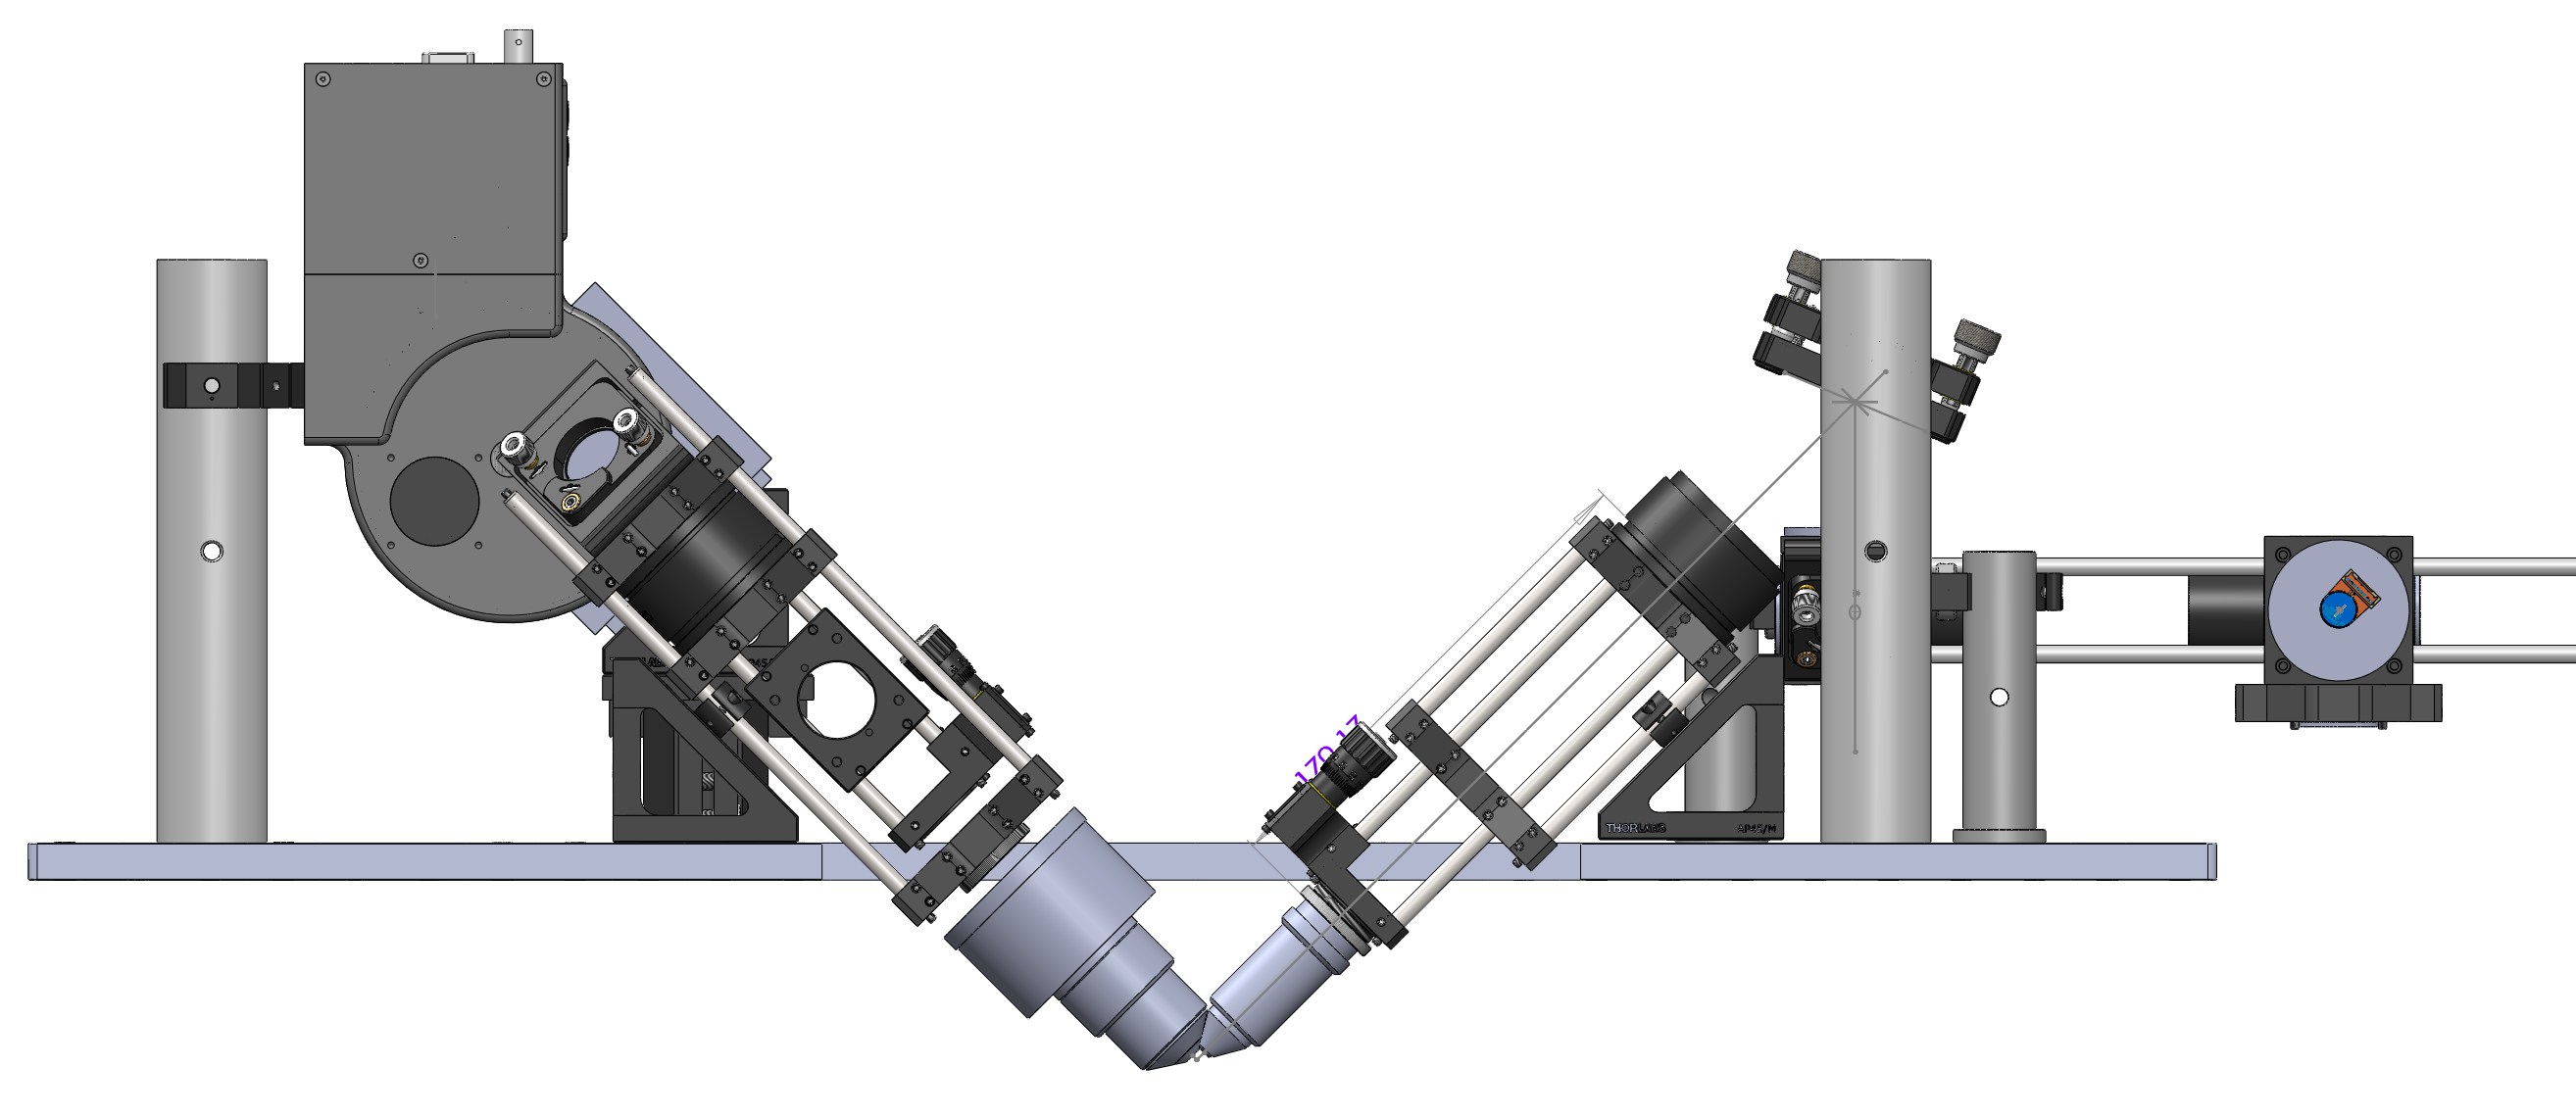
\includegraphics[width=1\linewidth]{./Raster/solidworks_design_front}
% \caption[CAD design of the \SI{45}{\degree} detection and illumination]{}\label{fig:solidworks_design_front}
% \end{figure}
%
% \begin{figure}
% 	\centering
% 	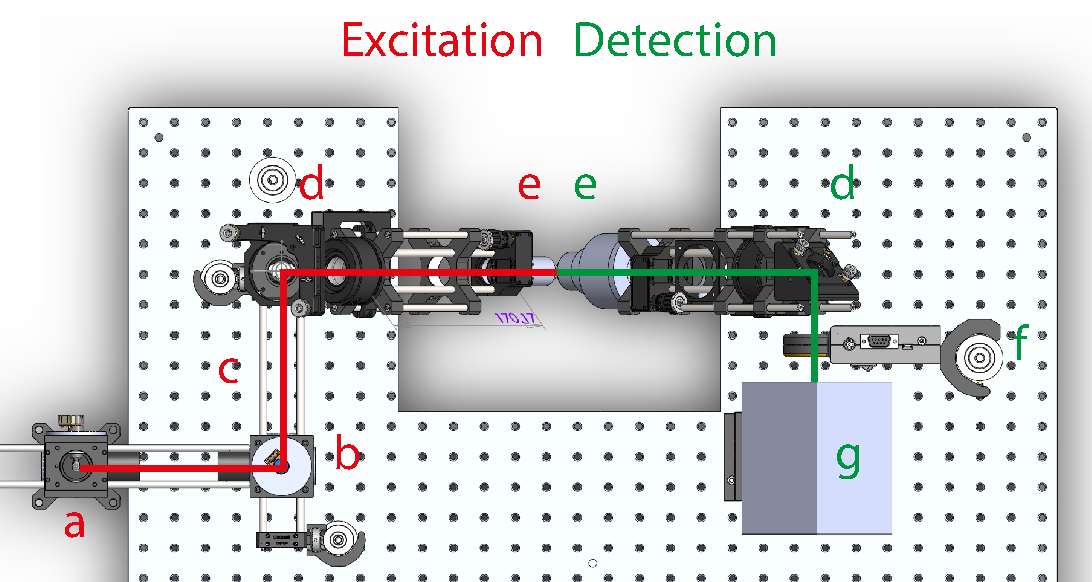
\includegraphics[width=\linewidth]{./soldiworks_top}
% 	\caption[Top down schematic of SPIM]{
%     (a) Scan mirror which creates the \gls{light-sheet}.
%     (b) Scan mirror in \(z\) for scanning volumes.
%     (c) Position of telecentric lens.
%     (d) Tube lens \emph{ITL200}
%     (e) Objective lenses, with green having an objective actuator.
%     (f) Emission filter wheel
%     (g) sCMOS camera
%     }\label{fig:soldiworks_top}
% \end{figure}

% \subsubsection{Scan Lens}
% %TODO something
% The scan lens was characterised (See appendix \ref{appendix:scanlens}) and placed at ... %TODO
% %See Appendix

\subsubsection{Light-sheet shaping} %Edited

% \newacronym{FOV}{FOV}{Field of View}
% \newacronym{sCMOS}{sCMOS}{scientific Complementary Metal-Oxide-Semiconductor}
% \newacronym{NA}{NA}{Numerical Aperture}

Using the Orca Flash v4 camera (with a sensor size of \SI[product-units=repeat]{13x13}{\milli\meter}) and a detection objective magnification of \SI{25}{\times}, produced a \gls{FOV} with an extension of
% a required \acrshort{FOV} of
\SI{520}{\micro\meter} in the \(x\) and \(y\) directions.
To match the confocal width of the illumination beam to the \gls{FOV} of camera sensor the illumination required \SI{0.15}{}~\gls{NA} at the back aperture of the illumination objective for \SI{561}{\nano\meter} light; providing a beam waist (\gls{light-sheet} thickness) of \SI{1.3(1)}{\micro\meter}, from Equation~\ref{eq:rayleigh}.
%\acrshort{NA}
To create an \gls{NA} of \SI{0.15}, for an objective of focal length \SI{20}{\milli\meter}, the back aperture would need to be filled by a beam of diameter \SI{6}{\milli\meter}.

Using an \emph{ITL200} tube lens with a \emph{Nikon A1} scan lens provided \SI{5.37}{\times} magnification (See Appendix~\ref{appendix:scanlens}), meaning the illumination objective back aperture would have been overfilled (\SI{7.52}{\milli\meter} beam diameter at the back aperture) and the usable \gls{FOV} too small.
To address this, an iris was placed at the back aperture of the illumination objective to allow for manual tuning of the \gls{NA}.
The downside of stopping down the back aperture, was that some light was discarded
\Gls{light-sheet} systems do not require large doses to function (\SI{\sim1}{\milli\watt}) and discarding a fraction of the light from the \SI{100}{\milli\watt} sources was not found to impede imaging.

%With a scan lens focal \SI{37.3\pm0.1}{\milli\meter}

%In the the old SPIM a standard NA of laser used was 0.15 which created a FOV of \SI{520}{\micro\meter} \footnote{The chip size of the sCMOS camera is \SI{13}{\milli\meter} and the magnification of the detection objective lens is \SI{25}{}$\times$ giving a field of view of \SI{520}{\micro\meter}} and a beam waist of \SI{1.3 \pm 1}{\micro\meter} (from equation \ref{eq:rayleigh}).
%To recreate a numerical aperture of \SI{0.15 \pm 0.05}, for an objective of focal length \SI{20}{\milli\meter}  the back aperture would need to be filled by a beam of diameter \SI{6}{\milli\meter}.
%Therefore the illumination laser needs to be magnified \SI{1.7}{}$\times$.
%Standard optical lenses are heavily quantised in terms of their focal length, a viable magnification for instance would be a \SI{160}{\milli\meter} , \SI{30}{\milli\meter} pair placed just before the flip mirror.
%A very sensible use of lenses would involve exploiting the lens that conjugates the SLM to the image plane, provided the lens were placed after the flip mirror and not before, which is possible if the focal length of the SLM is set higher than \SI{330}{\milli\meter} and therefore placed after the flip mirror.

%The beam waist was measured for one colour though each colour may require its own additional lenses as well as the overall demagnifying telescope.
%These additional lenses directly after the laser heads would compensate for any width and colour dependent variances in the field of view of the light sheet; the gratuitous additional optics (six lens for three uncorrected colours) may make this solution inviable as the only correction it will achieve is likely a small improvement in light sheet homogeneity.

\subsection{Detection}

%The optics surrounding the detection arm are far simpler than the excitation arm.
The detection lens used was a PlanAchromat \SI{25}{\times} high (\SI{1.1}{}) \gls{NA} objective, select the unparalleled lateral resolution for a water dipping lens that could fit the mechanical constraints of the \gls{light-sheet} system.
This was coupled to second \emph{ITL200} tube lens which imaged infinity corrected emission light onto the Orca Flash 4.0v2 detector.
% Before the detector there was
In the path between the detection objective a Prior Filter wheel housing emission filters (Semrock the \emph{442/647};
Chroma the \emph{ET605/70m} and \emph{ZT405/488/561/647rpc}) was installed to reject scattered illumination light.
%The emission filter is used to reject excitation light scattered from the sample, though this signal should be weak it is very difficult to correct for this digitally and so the filters are necessary.
%\subsubsection{Parfocal relay}

A further lens relay was added on the \gls{imaging optical rail} after the \gls{detection arm} turning mirror.
The relay comprised a tube lens and two objective lenses on a rotating turret.
This provided a par-focal solution for magnifying the imaging by \SI{2.5}{\times} (\emph{Olympus MPLFLN1.25x}) and \SI{1.25}{\times} (\emph{Olympus MPLFLN2.5x}) for \SI{62.5}{\times} and \SI{31.25}{\times} total magnifications respectively.
Using microscope objectives for the additional optical relay ensured that there were minimal optical losses as the lenses are designed for the weak fluorescent signal, as well as for minimal distortion and chromatic aberrations.
Imaging at \SI{62.5}{\times} magnification gives \SI{99.2}{\nano\meter} lateral sampling at the specimen plane.
The \glslink{Rayleigh length}{Raleigh} condition of the system, using \SI{561}{\nano\meter} light, is \SI{311}{\nano\meter} resolution.
%Meaning that
Therefore, at \SI{62.5}{\times} magnification, the system is sampled sufficiently for \glslink{nyquist sampling theory}{Nyquist criterion} (\SI{155.55}{\nano\meter})
%\footnote{which states that the sampling of a system needs be twice the bandwidth of a band-limited signal}
as the demagnified width of each \gls{photosite} (from the camera, at the specimen plane) is \(\frac{\SI{6.5}{\micro\meter}}{62.5}=\SI{104}{\nano\meter}\).

% under Nyquist sample criteon
%\section{Control}
\section{Software}

To control the \gls{light-sheet} microscope and acquire imaging data an open-source~\cite{russellSpimcontroller2017} software interface was developed, using \gls{LabVIEW}, to
% needed which would
send the appropriate electronic signals and serial commands.
%\subsubsection{Control}

\begin{figure}
    \centering
  \includegraphics{./controller_scheme} %TODO my own.
  \caption{Control schematic of the digitally scanned light-sheet microscope.
  All control signals are generated within \gls{LabVIEW} and distributed to the components.
  Components requiring fast signalling (lasers, scanning mirror, objective actuators) are synchronised by sending pre-built packaged signal trains.}\label{fig:control}
\end{figure}

% Comntrol schematic illustrator.

%We controlled this like that and here is a schematic of how it all connects:

\subsection{Signalling} %Edited slightly?

%\subsection{Implementation}
%Talk about synchornisaiton
Precise synchronisation is needed for confocal slit-scanning (Chapter~\ref{chapter:dualslit}) to be viable, as the time between the switching of active \gls{photosite} rows at \SI{100}{\hertz} for the Orca Flash v4 is \SI{\sim10}{\micro\second}. %TODO justify this better than surprise confocal?
%In the light-sheet system used here, t
This was achieved using fast electronics to send sets of packaged voltage waveforms through a National Instruments \gls{DAQ} module.
Once a \gls{TTL} 5V signal is sent to the camera, there is a delay of approximately \SI{10}{\milli\second} for the electronics to initialise on the camera.
During this window the \(y\) mirror, which creates the \gls{light-sheet}, and \(z\) mirror are pre-driven so that the mirrors are travelling at a constant velocity during the exposure window, giving a uniform illumination.
The time-point of the start of the exposure window was found empirically (\SI{9.8}{\milli\second} after camera triggering) by tuning this window until the illumination profile, under slit scanning, was uniform when visualised using fluorescent dye (Rhodamine).
During the exposure, a \gls{TTL} signal is sent to the requisite laser channel for illumination.
Once the exposure window is finished, the \(y\) and \(z\) mirror is sinusoidally returned to the start voltage for the next exposure (see \figurename~\ref{fig:slit_signals}); sinusoidal ramping helps protect the mirror against inertia-induced damage.

\begin{figure}
  \centering
  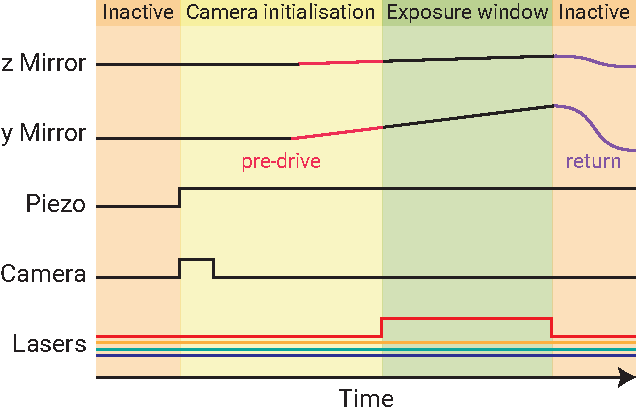
\includegraphics{slit_signals}
  \caption{The signals required to synchronise a rolling shutter in a digitally scanned light sheet.
  A pre-drive phase for the \(y\) mirror is needed to ensure the illumination profile of the light-sheet is uniform.
  The camera requires time to initialise the electronics and so a delay period is added within which the pre-drive of both mirrors is performed.
  Both mirrors are sinusoidally returned to their start position ready for the next acquisition.
  }\label{fig:slit_signals}
\end{figure}

Control and synchronisation of the filter wheel and XYZ translation stage was achieved using \gls{RS232} serial commands, as precise timing was not needed and direct feedback on the status of the stage and filter was desirable. %from the controller on where the stage and Filter

%TODO Basic overview.
%Sample Area
%	Requirements and Limitations of the samples to be used
%Illumination
%
%Detection
%Image Acquisition
%	Hardware interfacing, software control and end-user interface

%\subsection{Image Acquisition: Software Design}

%TODO discuss aims of software and version control

\subsection{\gls{LabVIEW} control software}

A modular, extensible and easy-to-use software solution was needed to control the \gls{light-sheet} microscope.
\gls{LabVIEW}, a graphical programming language with an emphasis on electronic systems control, was used.
\gls{LabVIEW} provides a wide library of drivers and libraries for interfacing; in particular the Orca Flash v4 has \gls{LabVIEW} drivers for direct control of its reader functionality, including the requisite commands for confocal slit scanning.

\subsubsection{\gls{LabVIEW} architecture}

% LabVIEW is a graphical programming software package designed to produce simple, modifiable, user-friendly software in science.
% LabVIEW provides a wide library of drivers and libraries for hardware interfacing in science.
% Due to LabVIEW's modularity and fast development environment it is ideal for producing software for a microscope under development as any new hardware can be quickly and easily implemented and not necessarily by the original software writer.

It was required that the components within the microscope were interfaced in a parallel manner as well as controlling and interfacing with each other (e.g. the XYZ controller triggering the capturing of a image volume).
The software controller was engineered using a \glslink{producer-consumer architecture}{producer} where each \glslink{producer-consumer architecture}{consumer} was a parallel \gls{state machine}.
The \glslink{producer-consumer architecture}{producer} will receive front panel inputs, then convert and pass those commands on to the \glslink{producer-consumer architecture}{consumer}s.
Using a \gls{queueing architecture} ensured that command flooding and \gls{race conditions} are avoided, and the consumer loop can be self regulating.
%This ensures that command flooding and race conditions are avoided and the consumer loop can be self regulating.

The commands were packaged as a bundle.
The first part being an enumerated type which changed the \emph{state} of the \glslink{producer-consumer architecture}{consumer}; the second being the necessary front panel data which informed the consumer on any updates to the states (e.g.\ camera exposure).
By using this queuing architecture, consumers can then communicate with each other whilst functioning independently.

%
% %A well planned, modular and user-friendly interface is very important whenever creating hardware-user interfaces.
% %In the case of the new microscope this software needs three different components.
% %The first is t
% The software needed to several modules: the Camera control software, which controls the detection arm of the microscope, needed to
% %; this software needs to
% allow a user to save two and three dimensional stacks of images and still be accessible to change and upgrade as more and difficult biological questions were to be addressed.
%
% A XYZ stage controller controller for the stage which that could interface with the camera software (to take images for large area scanning for instance)%. as well as being user friendly enough to accurately control the XYZ stage.
% and finally, a waveform generator to control and synchronise the scanning mirrors, focus piezo and potentially tunable lenses.
% These software also needed to be designed as modules so that a user could use each independent of the others.
% To satisfy these criteria LabVIEW was chosen as the programming environment to be used.

%\subsubsection{Camera module}


% \subsubsection{Queuing}
%
% When interfacing with hardware a key challenge programmers face is how to mitigate command flooding at the device.
% A user may for instance want to send several commands in a linear fashion, but the device may only be able to successfully implement one or none if it crashes with overload or misinterprets the command as it is processing another.
% LabVIEW offers a queueing architecture where a programmer can send a command into a queue which will operate something, be it a real device or a construct within the software.
% This queueing opens a myriad of possibilities.
% The programmer can not only queue an infinite line of commands but also remove duplicate commands, truncate a command queue, change the routine of operation to a first in first out (FIFO) routine rather than first in last out (FILO) or even enforce that only one command can exist it the queue at any time.
%
% \subsubsection{Simple State Machine}
%
% A state machine is a fundamental computing architecture which can contend with a great deal of complex programmatical challenges.
% A common example of a state machine is a vending machine: when left alone the vending machine keeps its state (usually an enumerated variable) as idle.
% If a user adds a coin it begins a routine of \textit{add currency to running total}.
% If a user presses dispense the next state will check the running total of currency, if the currency is too low the current state then changes its next state to return coin or any other operation.
% It is a very simple method of keeping a clear routine within the program rather than any abstractions that would occur if programmed otherwise.
%
%
% \subsubsection{Producer Consumer}
%
% %In LabVIEW the combination of queueing and state machines facilitates the producer consumer concept, whereby the producer is an independent parallel routine which can queue commands for a consumer.
% %The most simple template for this is an event driven producer recommended as the start of any LabVIEW routine, whereby the event loop collects commands from the Graphical User Interface (the front panel in LabVIEW).
% %This producer then produces commands to be sent to the consumer loop which processes them.
% This ensures that command flooding and race conditions are avoided and the consumer loop can be self regulating.
% Crucially, queued commands can come from more than one entity in this style of environment.
% Not only can commands from the front panel control the consumer, but also commands (if correctly written) can arrive from sources such as the internet, other devices, or other front panels within LabVIEW.

% \begin{figure}
% \centering
% 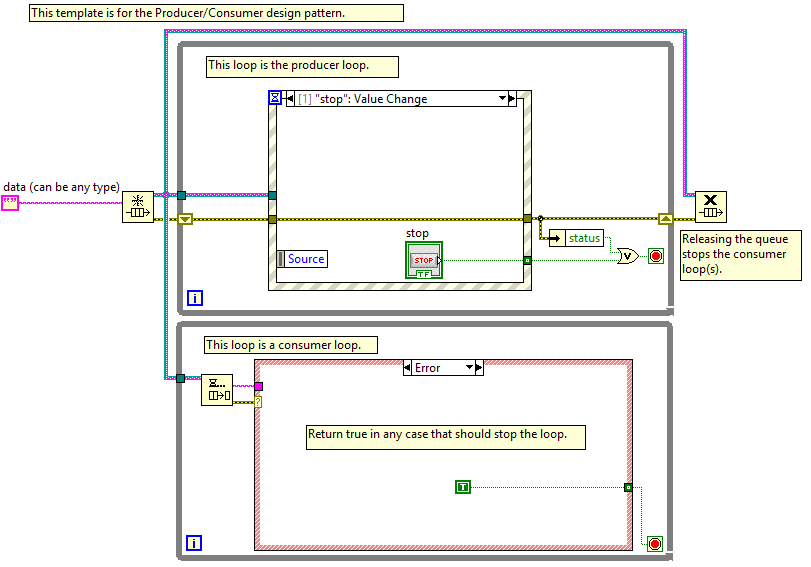
\includegraphics[width=0.8\linewidth]{Figures/standard_pro_cons}
% \caption[LabVIEW Producer Consumer Template]{A producer consumer template provided by national instruments.
% The top loop is an event driven (user front panel input) producer loop, the bottom loop consumes these commands and acts accordingly.}
% \label{fig:standard_pro_cons}
% \end{figure}

\begin{figure}
    \centering
    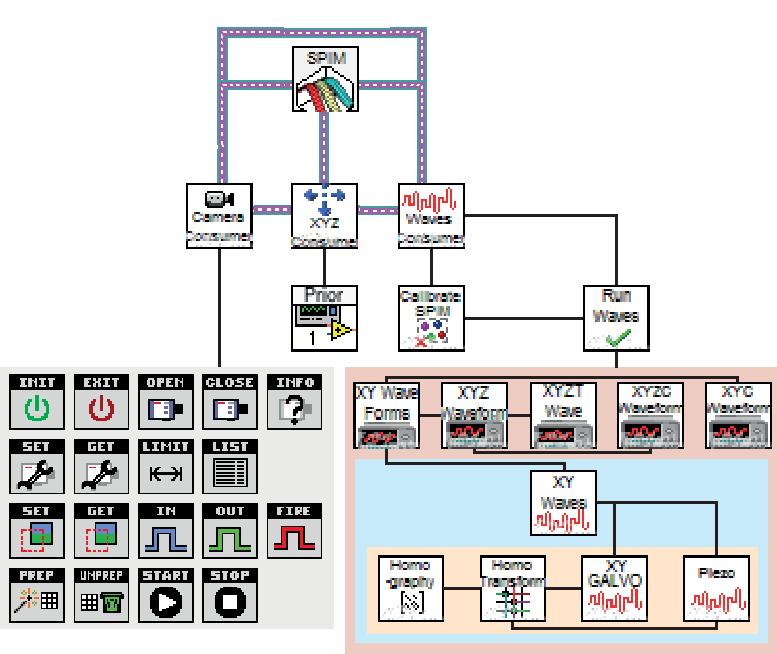
\includegraphics{/software_layout}
    \caption{Schematic diagram of the dependancies of each routine in the \gls{LabVIEW} software (\emph{SPIM}, the kernel) that runs the light-sheet microscope.
    The \emph{Camera consumer} and \emph{XYZ consumer} package the Hamamatsu capture (grey) and Prior iScan libraries (\emph{Scan}) respectively.
    The \emph{Waves consumer} packages the signal generating routines (red) and drives the resultant signals to the DAQ board using \emph{Run waves}.
    Each of the waves routines (red) are concatenations of \emph{XY waveforms}, which itself relies on \emph{XY waves} (blue) generates signal trains from calibration coordinates and front panel data.
    \emph{Homo-graphy} and \emph{Homo transform} (orange) take calibration coordinates to then inform \emph{XY Galvos}.\\
    The purple connections represent \gls{LabVIEW} queue connectors; each purple-connected module, other than the main kernel (SPIM), was an independent queued consumer state machine.
    State changing commands were added to each module's queue and could be received from any other connected module.
    This allowed for conditions such as the \emph{XYZ controller} being able to request \emph{Camera consumer} for an image or volume to be recorded using a simple \glslink{enumerated type}{enumerated} command.
    }\label{fig:software_layout}
\end{figure}

\subsubsection{Kernel}

The kernel stores the acquisition settings and initiates all the queues to be sent the the sub modules, \textbf{Camera}, \textbf{Waveform Generator} and \textbf{XYZ Translator}.
All acquisition settings and properties are converted into \gls{enumerated type}{enumerated} state machine commands.
Acquisition modes are organised into imaging orders, such as \emph{XYZ}, \emph{XYZC}, \emph{XYCZ}, \emph{XYT}; where \emph{XY} is a single frame, \emph{Z} is an iteration axially, \emph{C} is the colour channels selected, and \emph{T} is the time course selected.
Each of the dimensions (\emph{XYZT}) are governed by the parameters \emph{Start}, \emph{Step}, \emph{Range}; where start is the initial position or time; step is the step size, meaning spatial resolution or temporal resolution; and range is the range over which the dimension covers, spatially or temporally.
For colour, a \(2\times n\) array of enumerated typed is constructed for laser line and respective filter wheel position choice.
The kernel also stores the calibration coordinates (see Chapter~\ref{chapter:homography}) sent from the calibration module.
All of the
%these
settings can then exported as XML files and may be reloaded later.
%The kernel also manages the saving and loading of acquisition settings.


\subsubsection{Camera module}

The camera module consists of two consumers.
The first
% module runs a
consumer initiates and destroys the camera communications; as well as
%There are also
soft update states (for instance changes to \gls{exposure time}), and hard update states
(for when an acquisition setting requires the camera link to be unloaded, such as changing the \emph{sensor mode} which controls the shutter directions).
The difference between hard and soft updates is poorly documented and the categorisation of was found empirically.

The second consumer loop exists within the the camera module to handle saving and displaying of image data.
This consumer has two settings: the first receives queued image arrays directly from the camera, this is used for live preview mode and small image sequences such as single volumes; the second reads and converts image files from the file-stream of the camera.
The latter mode does not drop frames as the camera is streaming data directly to the hard drive, provided the read and write streams of the hard-drive do not overflow.
The single frame acquisition mode will also not drop frames due to their sequence being queued, but, there may be a delay between the presented image and the live view at high frame rates.

\paragraph{Virtual slit}
%{Virtual slit}

The virtual slit for confocal slit scanning was addressed in the camera's hardware directly using hex address \(\times 400210\).
Mode 1, sets the camera to full frame and mode 12, slit scanning.
Once the mode is set the line interval (\(\times 403850\)) and slit exposure (\(\times \text{1F0110}\)) is set according to the equation:

\begin{align}
    \text{Slit exposure} &= \frac{\text{Exposure} \times \text{Slit width}}{\SI{10}{\milli\second} + \text{FOV}_y + \text{Slit width}} \\
    \text{Line interval} &= \frac{\text{Slit exposure}}{\text{Slit width}}
\end{align}

\subsubsection{Waveform module}

The waveforms module handles all signalling for the \gls{DAQ} board (four laser lines, piezo, Y mirror, Z mirror, camera trigger, filter wheel).
The waveforms are constructed from the acquisition settings %for digital and analogue signals, which
and are forced to synchronise using propagation error values
\footnote{\gls{LabVIEW} is a data flow language so synchronisation is controlled using propagating variables and commonly using the error output of the function.}
.

The camera and lasers were addressed using digital (\gls{TTL}) signals which are hardware limited between \SIrange{0}{5}{\volt}.
Voltages to the objective actuator and scanning mirrors were software limited between \SIrange{0}{10}{\volt} and \SIrange{-10}{10}{\volt} (\SI{10}{\volt} = \SI{100}{\micro\meter}) respectively, to prevent damage to the electronics.
The objective actuator was positioned linearly, by voltage, using the conversation \SI{10}{\per\volt\micro\meter}; with \SI{16}{\bit} voltage resolution from the \gls{DAQ}, this gave an addressable axial resolution of \SI{1.52}{\nano\meter}, which was \SI{4}{\times} larger than the reported closed loop resolution (\SI{0.4}{\nano\meter}) of actuator.
Achieving the full resolution would have required addressing the actuator using serial commands which would have been too slow for the required imaging modes, such particle tracking.
As such the resolution trade-off was accepted.


%  with the digital.
%To create the wavesforms, XY wavefroms are concantThe waveforms are generated by concatenating
%
% \subsubsection{XYZ stage and filter wheel module}
%
% The XYZ module reads and writes XYZ stage positions and filter wheel positions using \gls{RS232}.
% For imaging, a list of locations to tour was added with the ability to the trigger current kernel acquisition mode in the kernel at each location visited.

\subsubsection{Calibration module}

The calibration module set the microscope to live image preview mode with direct user control over the objective actuator voltage and mirror voltages.
The module was used to set the limits of the usable volumetric FOV and match the focus of the objective to mirror positions, discussed in detail in Chapter~\ref{chapter:homography}.

\section{Specification review}

\begin{figure}
  \begin{subfigure}
    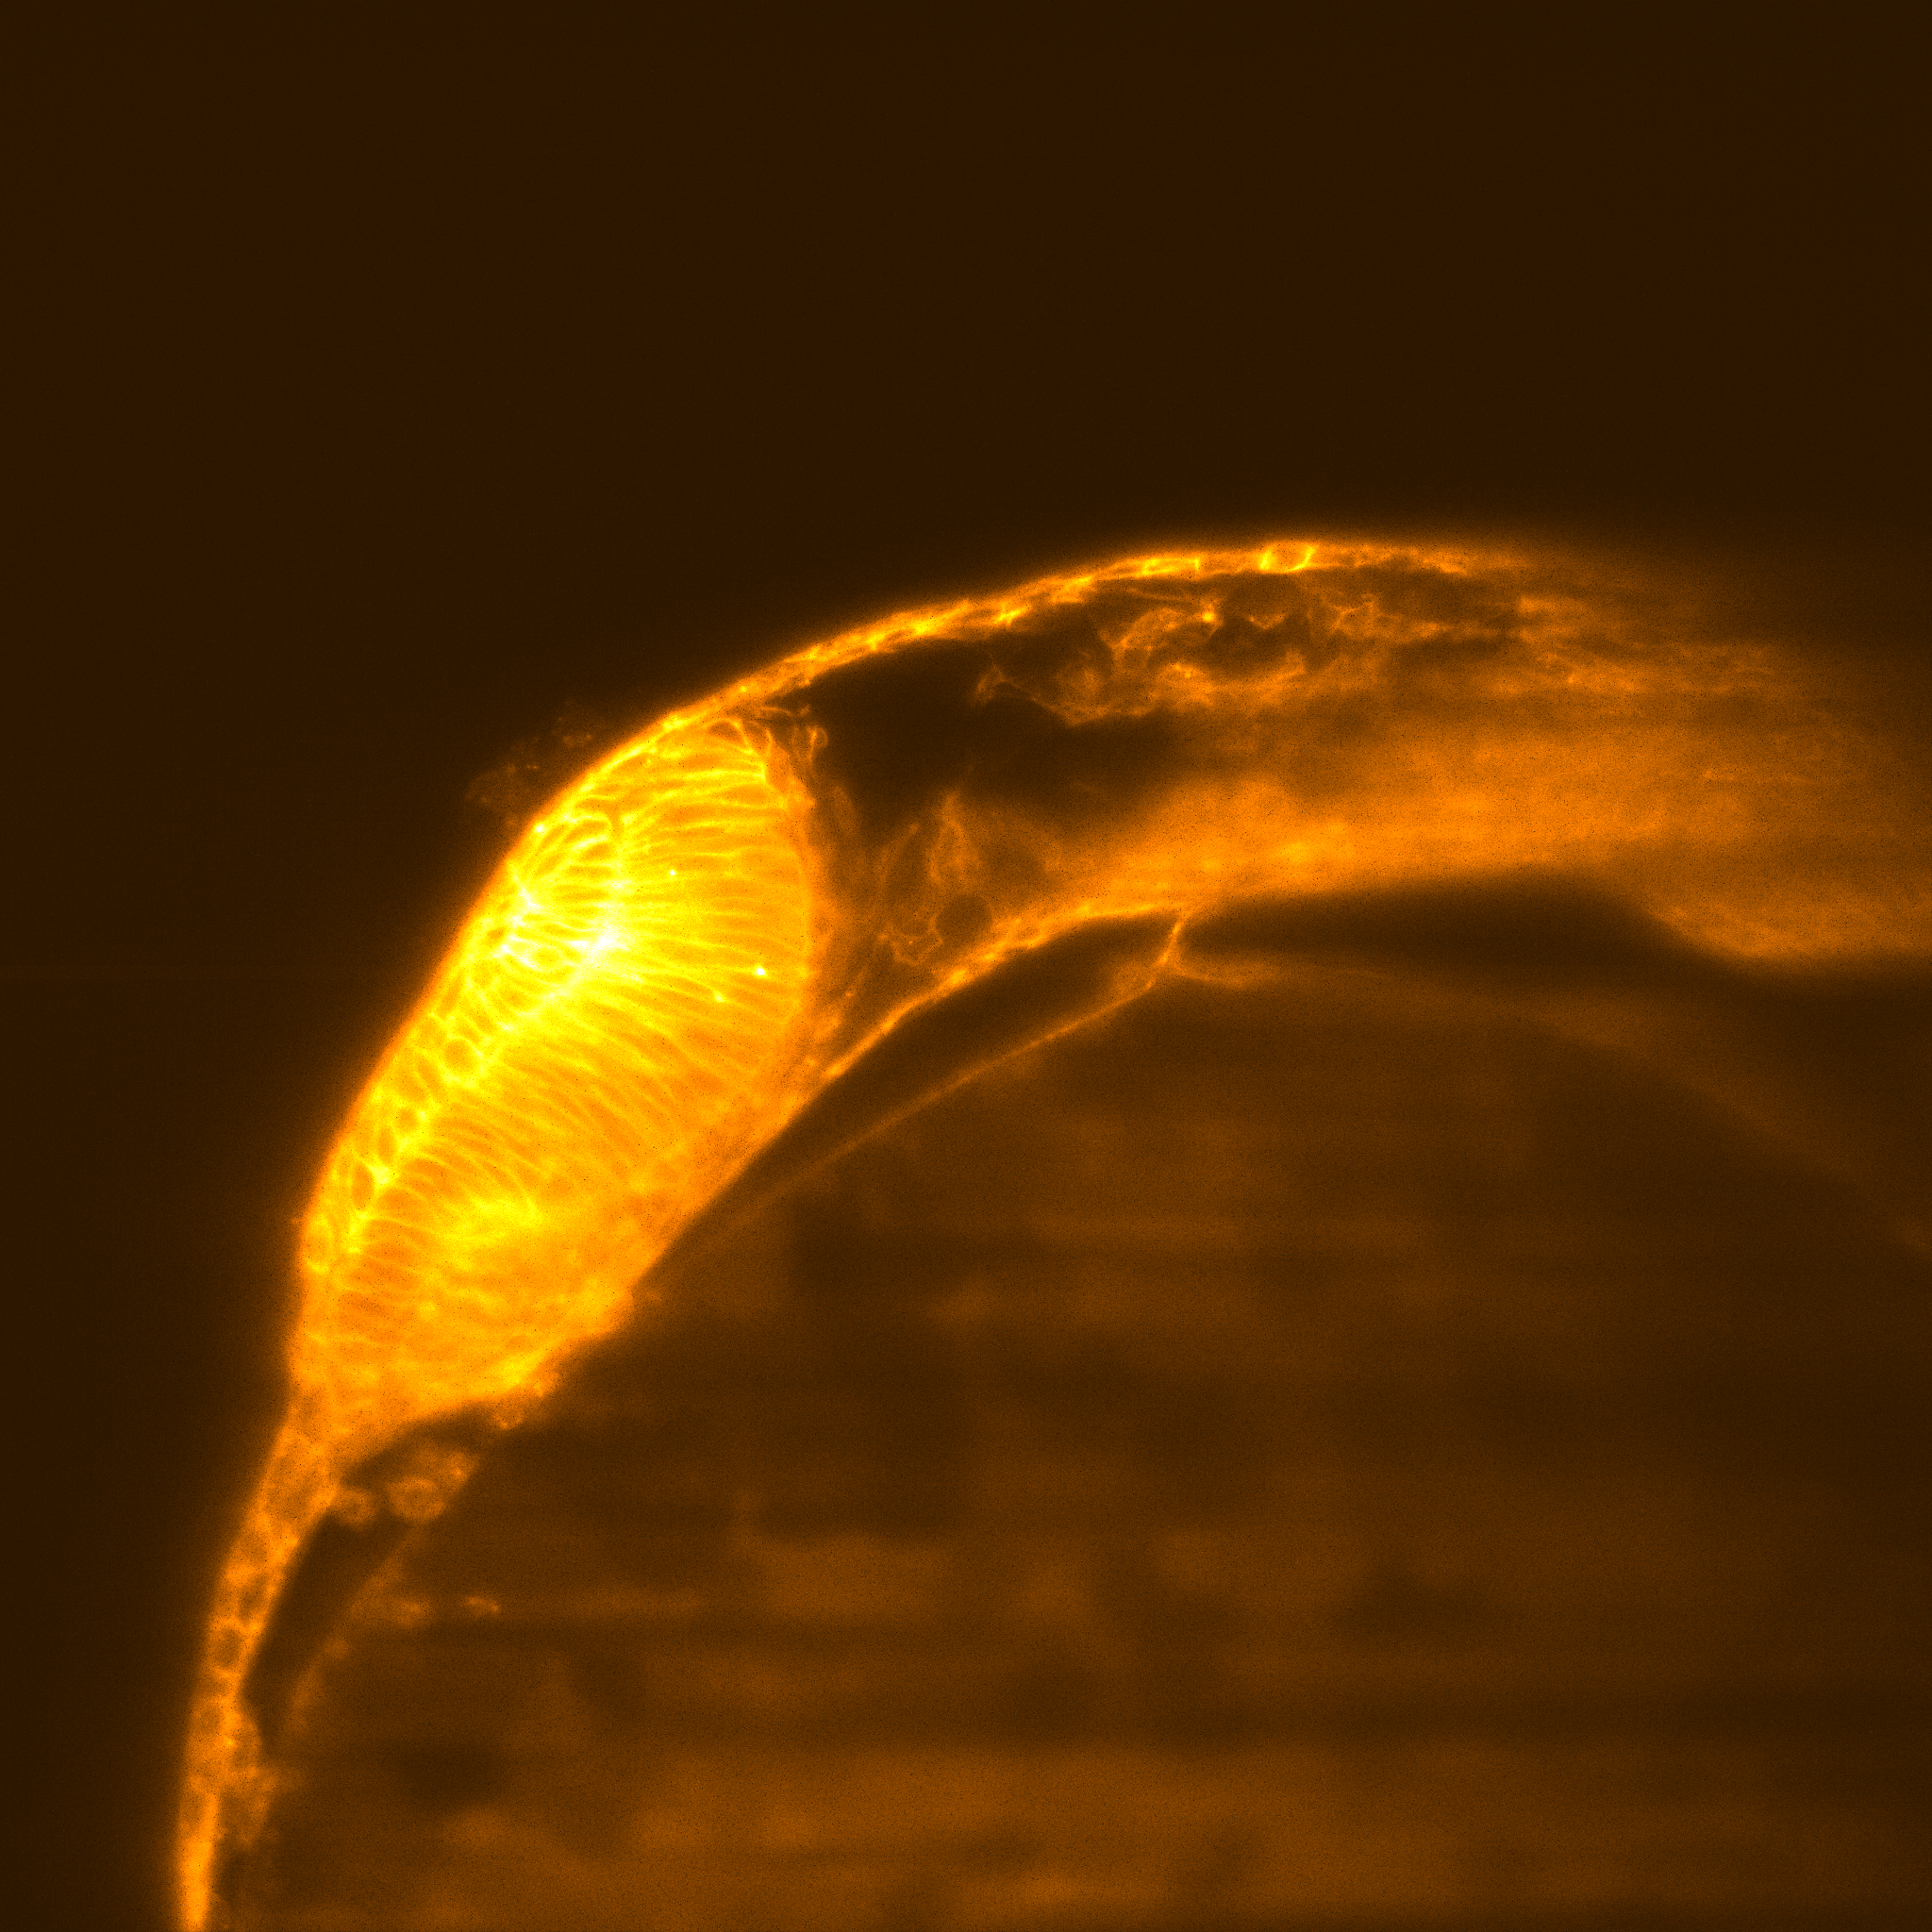
\includegraphics{zfish_48hr_eye_magneta}[t]{0.4\linewidth}
    \caption{\SI{48}{\hour}, \gls{zebrafish} eye}
  \end{subfigure}~
  \begin{subfigure}
    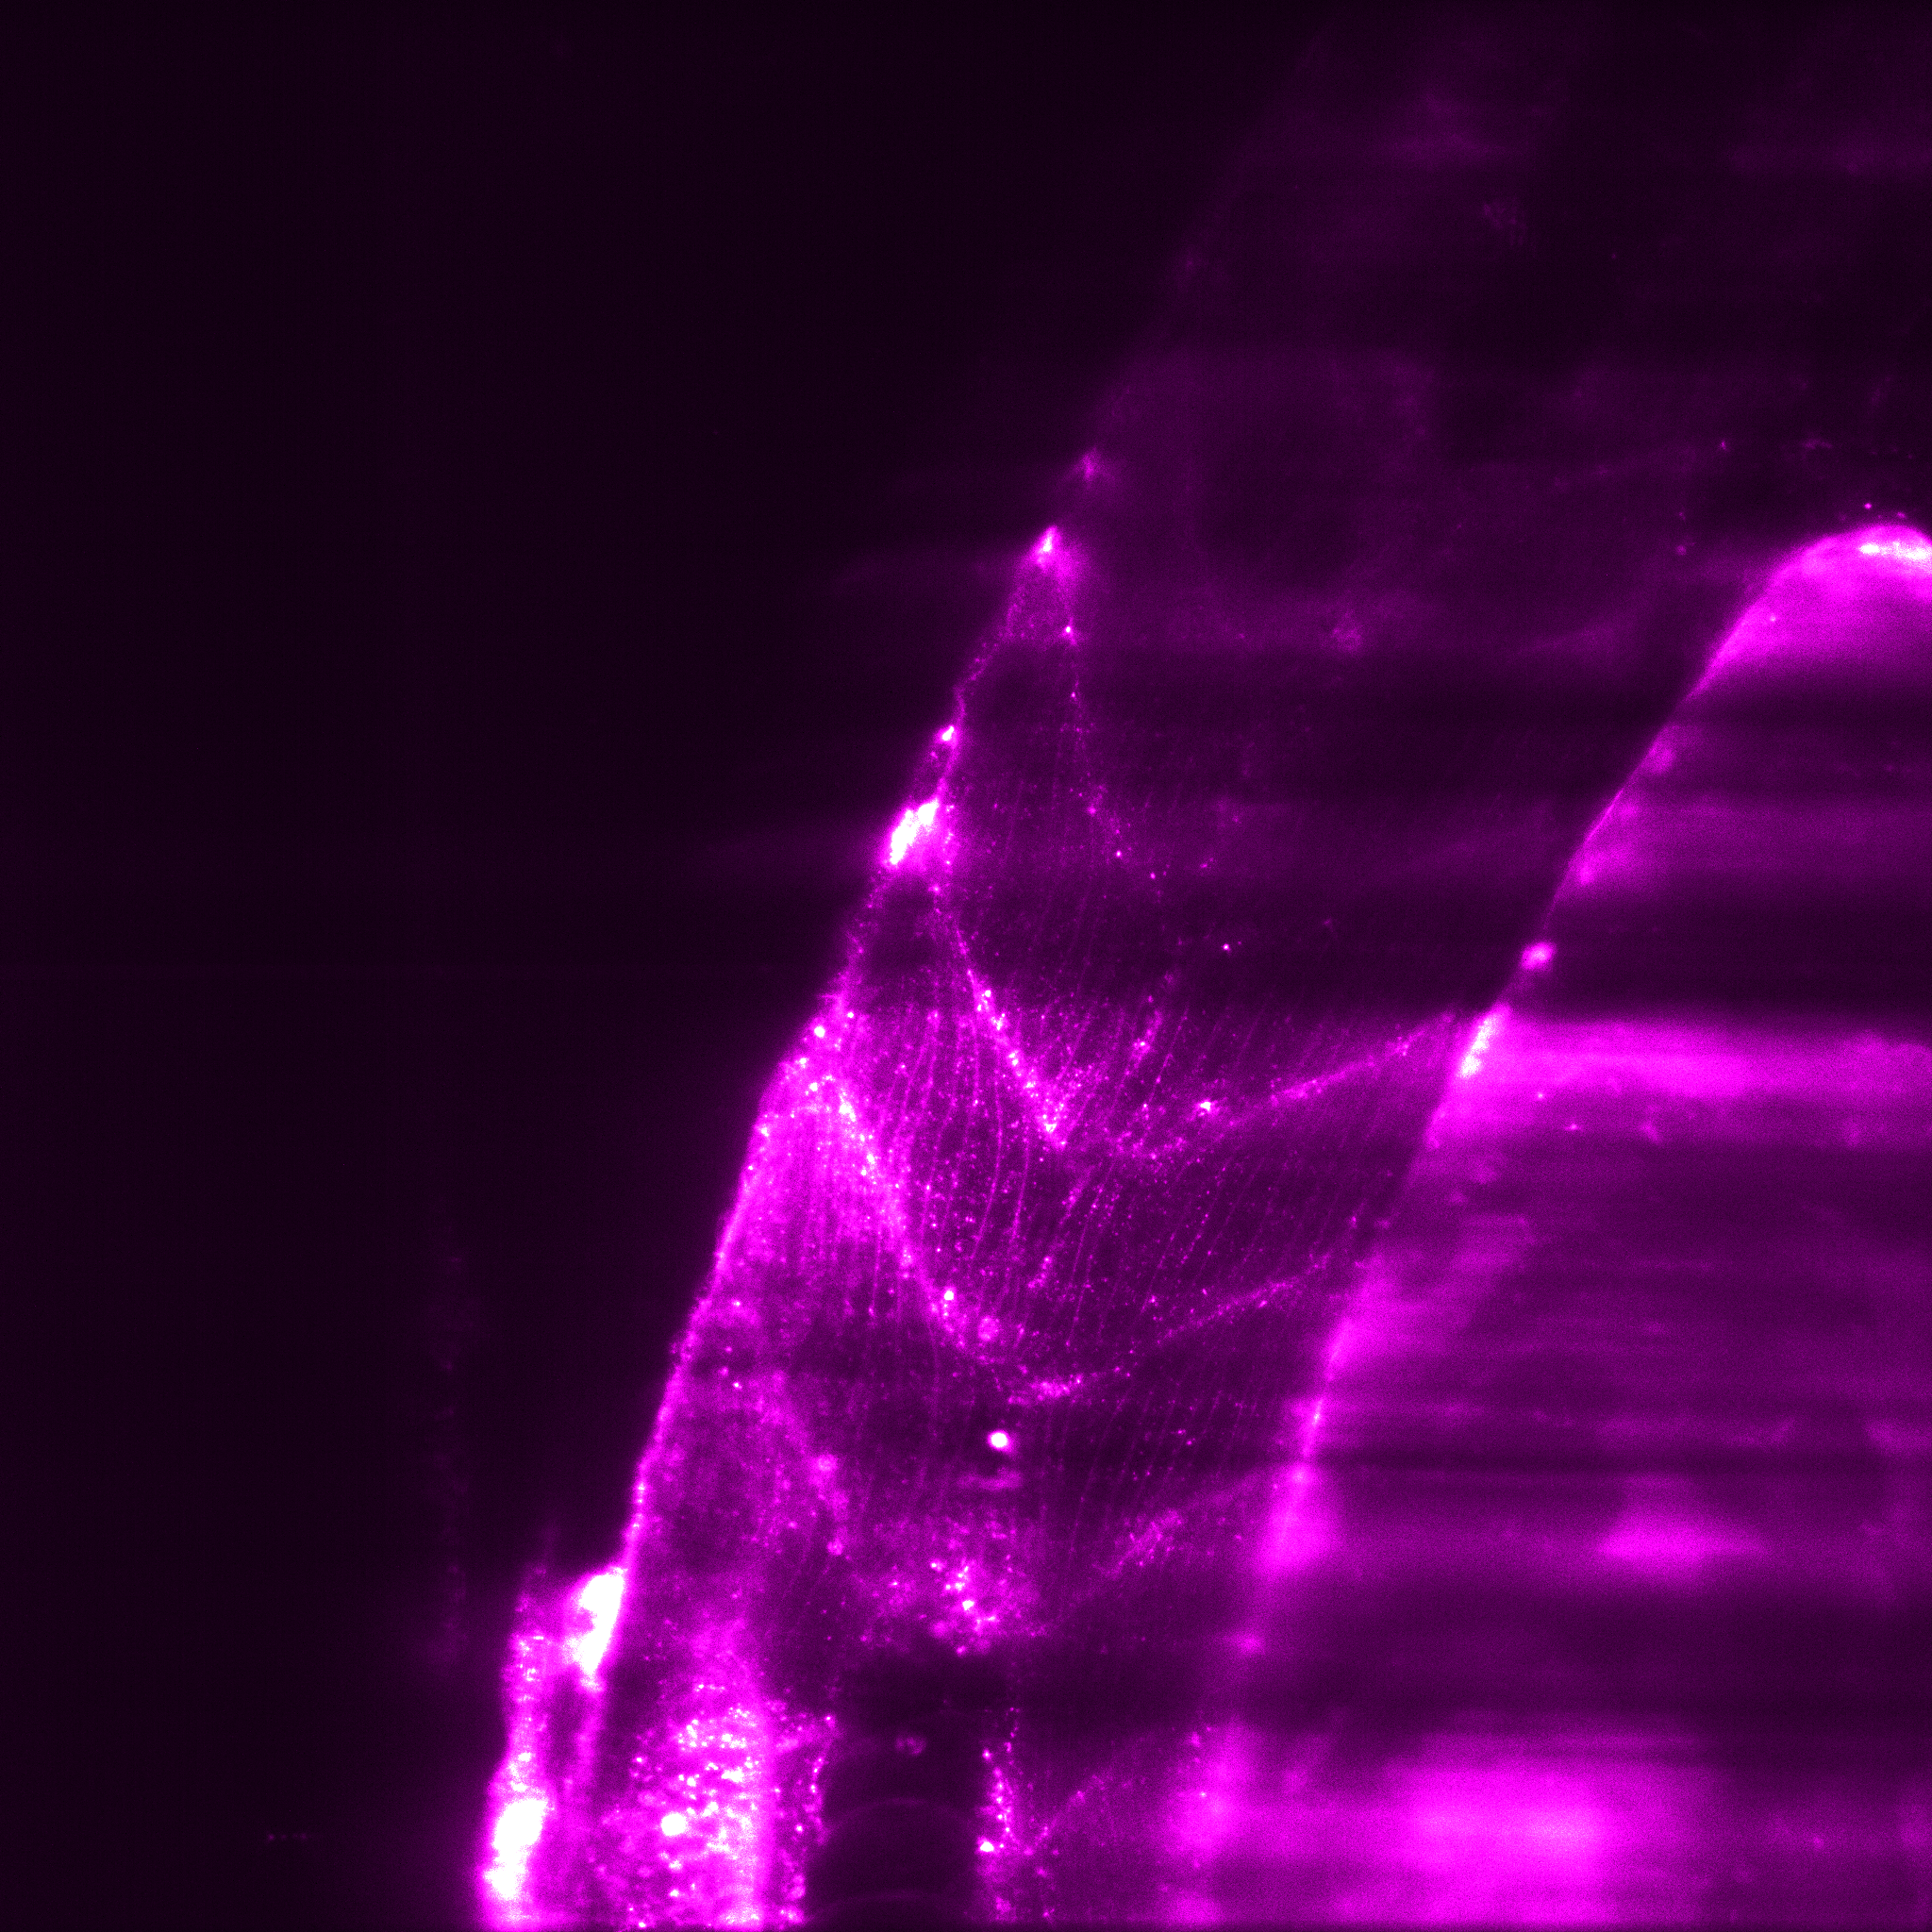
\includegraphics{zfish_48hr_noto_magenta}[t]{0.4\linewidth}
    \caption{\SI{48}{\hour}, \gls{zebrafish} notochord}
  \end{subfigure}
  \includegraphics{/path/to/figure}
  \caption{Preliminary images of zebrafish produced from the light-sheet microscope designed and built in this work.}\label{fig:zfish_pretty}
\end{figure}

A \gls{light-sheet} microscope was built to the design specification in Section~\ref{sec:specification}.

\paragraph{\ref{item:volumes}. Fast volumetric imaging}
Fast volumetric imaging (see \figurename~\ref{fig:zfish_pretty}) was achieved using a pair of optically relayed scanning mirrors to rapidly sweep a virtual light-sheet through volumes.
A Piezo objective actuator was used to maximise the axial speed at which volumes could be acquired.

\paragraph{\ref{item:colour}. Multi-colour volumetric imaging}
Four laser lines were used with a 6-port fast filter wheel on the \gls{imaging optical rail} and
%the illumination lines were \gls{TTL} trigged diode lasers
simultaneous \gls{TTL}-control of diode laser illumination
to allow for fast colour switching, to image multi-colour volumes rapidly.
The limiting step for speed was the filter wheel, though multi-notch filters were used for bespoke cases needing maximal colour switching speed (in which case only the \gls{Laser} diodes were switched to change colour channels).% be used in bespoke cases

\paragraph{\ref{item:mounting}. Capacity for multiple methods of sample mounting}
An XYZ translator was mounted well below the two dipping objectives.
This allowed for traditional mounting strategies, such as agarose filled \gls{FEP} tubing, as well as bespoke solutions for difficult samples, such as live cells.
The translator enabled precision positioning as well as large FOV imaging through positional mosaicing.
Chapter \ref{chapter:chamber} discusses, in detail, the sample mounting procedures used.

\paragraph{\ref{item:scales}. Multiple magnifications}
A par-focal relay using microscope objective lenses was inserted in the detection path to allow for two FOVs to be chosen from. This allow for the imaging of a large gamut of biological samples, from the cell up to the organism.

\paragraph{\ref{item:illumination}. Options for exotic illumination development}
A beam splitter was placed on the lower optical breadboard before reaching the scanning mirrors above. Using flip mirrors and beam dumps enabled the option of a dual-beam illumination or an exotic illumination from the SLM found on one of the arms.

\paragraph{\ref{item:software}. User-friendly and extensible software scheme}
\gls{LabVIEW} was used to create a modular system for the control software.
By using an appropriate architecture, as detailed above, modules could interact freely and run in parallel.

The following chapter will expand on the signal generation presented in this chapter in an attempt to optimise and maximise co-planarity between the imaging and illumination planes.

%The software was designed such that it could be ported to other systems with minimal re-programming

%
% % %The Prior controller interfaces with software via an \gls{RS232} protocol.
% % %Provided with the stage is a library of routines within LabVIEW that package the correct \gls{RS232} commands in a LabVIEW friendly format.
% % %These were then incorporated into $XYZ\_Controller.vi$ producer consumer loop.
% % %This time however the stage controlling consumer loop was a slave to the consumer that handled front panel inputs.
% % %This was because the controller is cantered about the list of positions.
% % This list sends positional commands to the stage, but also requires functions such as: clearing the positional list; adding current position to the beginning or the end of the list; controlling the delay between positions and sending save image volume commands.
% %
% % For filter wheel control, \gls{RS232} commands were synchronsied with the \gls{TTL} triggers from the Waveforms module.
% % A small listening routine was written to intercept triggers sent to a false channel, these triggers were then converted to filter wheel positions.
% % The maximum settling time for non-adjacent filters is \SI{40}{\milli\second}, so a comparable delay was added into the imaging routine to compensate for filter switching.
% % \gls{RS232} commands require a comparable amount of time in handshaking, so attempting to check if the filter wheel was in the correct place before continuing would not be faster.
%
% % drop frames, but has the potential to
%
% % Camera modules
% % Saving to ram or harddisk. Involved another consumer slave to take queued images from the camera consumer-cum-producer.
% % The camera required an idle state so as not to hang when no commands had been sent
% % Hard and soft update states, for camera.
% %% Virtual slit
% % Hex values, 10 ms delay
% % Waveform modules
% % Synchronised waveform sending
% %
% % Image
% % XYZ Module
%
% %\subsection{Camera module}
%
%
%
% % Camera.vi was designed to be the main running loop of the software environment.
% % That said, all of its functionality has been designed so that each function could be addressed by properly accessing the queue named \textbf{Camera}.
%
% %\subsubsection{Front Panel}~
%
% % Care was taken to ensure that the user experience of the Camera.vi was well received and fundamentally simple.
% % A simple user experience can both necessitate the microscope to be used by a lay individual for simple exercises as well as allow experienced users to access more advanced aspects of the microscope.
% % % The imaging area of the Camera.vi was therefore set within a scalable box, so that setting on the left and image recording settings would shift away.
% % The settings on the left were organised into categorised tabs and initialised with camera defaults so that a complicated set up procedure is unnecessary.
% % See Figure \ref{fig:camera_frontpanel} for depiction.
%
% \begin{figure}
% \centering
% 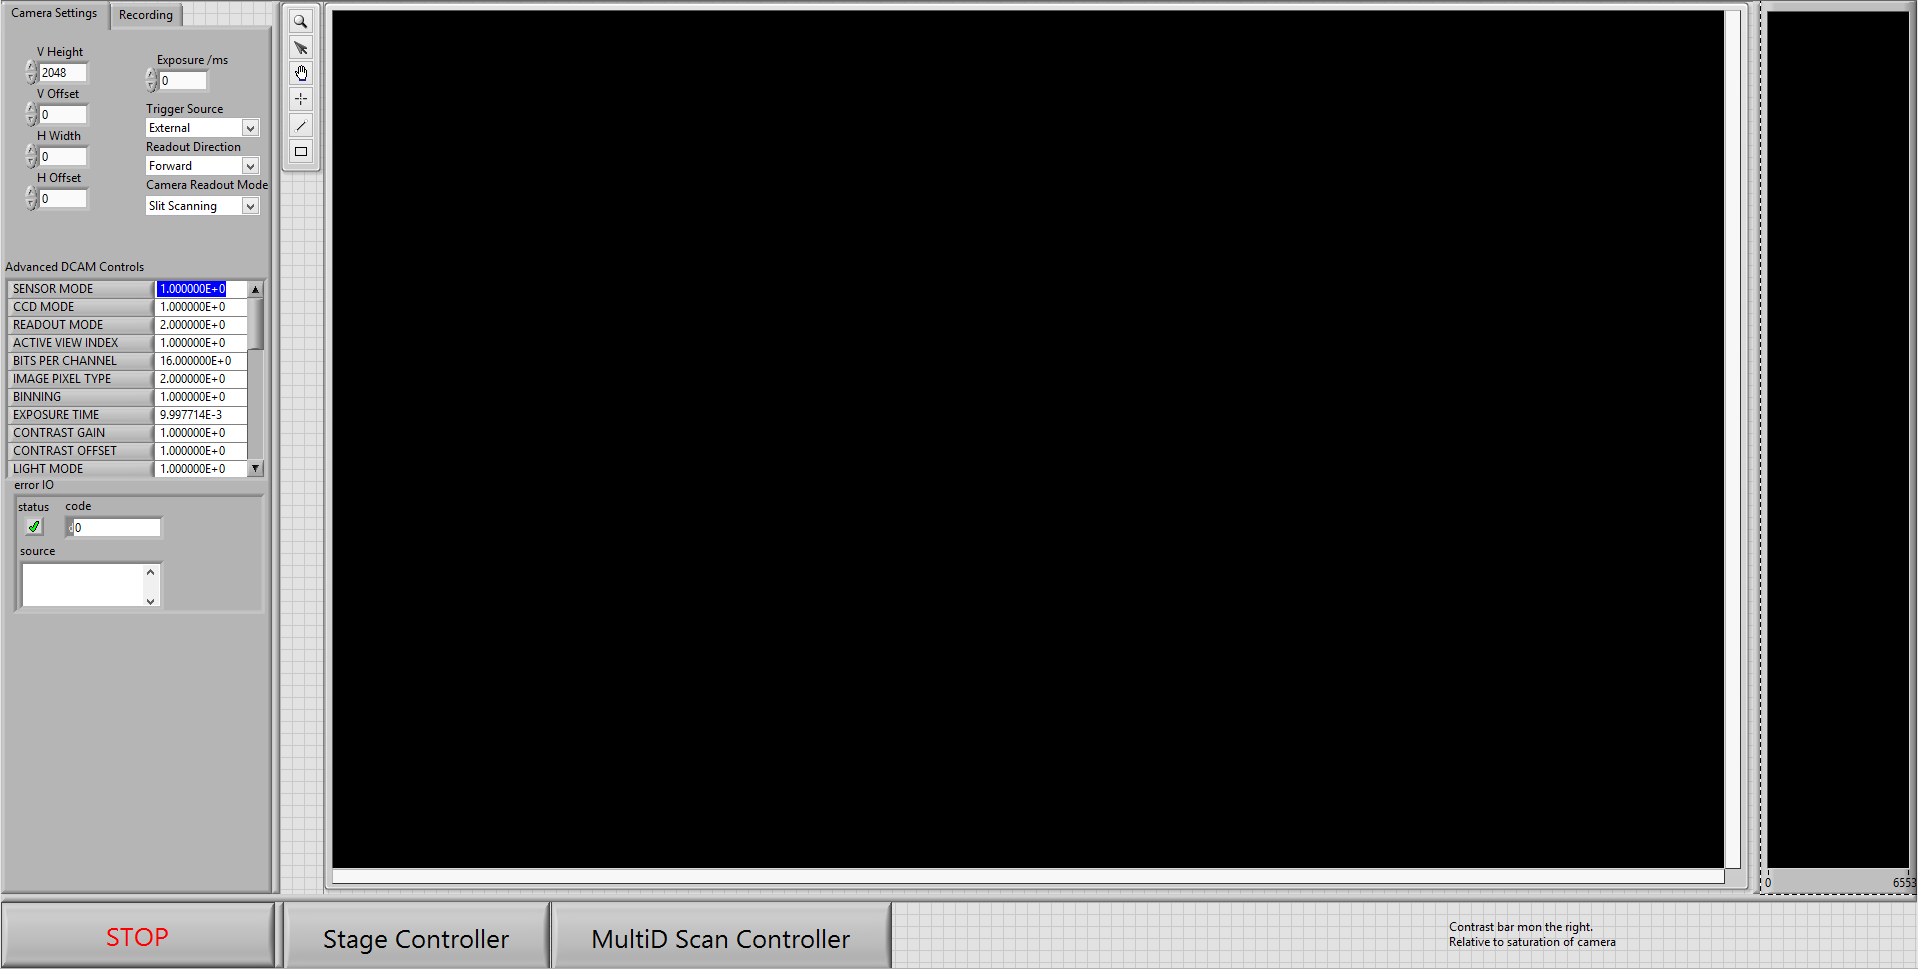
\includegraphics[width=\linewidth]{Figures/camera_frontpanel}
% \caption[Front Panel of Camera.vi]{Front panel interface of the Camera.vi routine.
% On the left is all the information and camera tools a user should need, tabbed into categories.
% At the bottom options to stop the program and open other supplementary programs.
% On the right an intensity histogram so the user can clearly see if the image being produced is making good use of the full dynamic range of the camera or to monitor if the camera is being saturated.}
% \label{fig:camera_frontpanel}
% \end{figure}
%
% % \subsubsection{Back Panel}~
%
% %The camera itself is split into three states: \textbf{init}alisation, \textbf{active} and \textbf{deinit}ialisation.
% %This structure was used so that collaborators could easily contribute as required.
% %Within \textit{active} the full producer consumer architecture runs.
% %The top loop typically seen as the producer takes all the front panel commands possible, passing the commands with any relevant numbers or information) in a bundled structure) to the camera control consumer loop.
% % %This loop then updates the camera as required and passes any images it received to a third slave loop which displays images as well as saving them to disk.
% % This secondary loop uses a limited queue so that is for any reason LabVIEW cannot handle the output of the camera then frames will drop when in preview mode to compensate.
% % Two disk saving modes were implemented in case of extreme uses of the camera.
%
% \begin{figure}
% 	\centering
% 	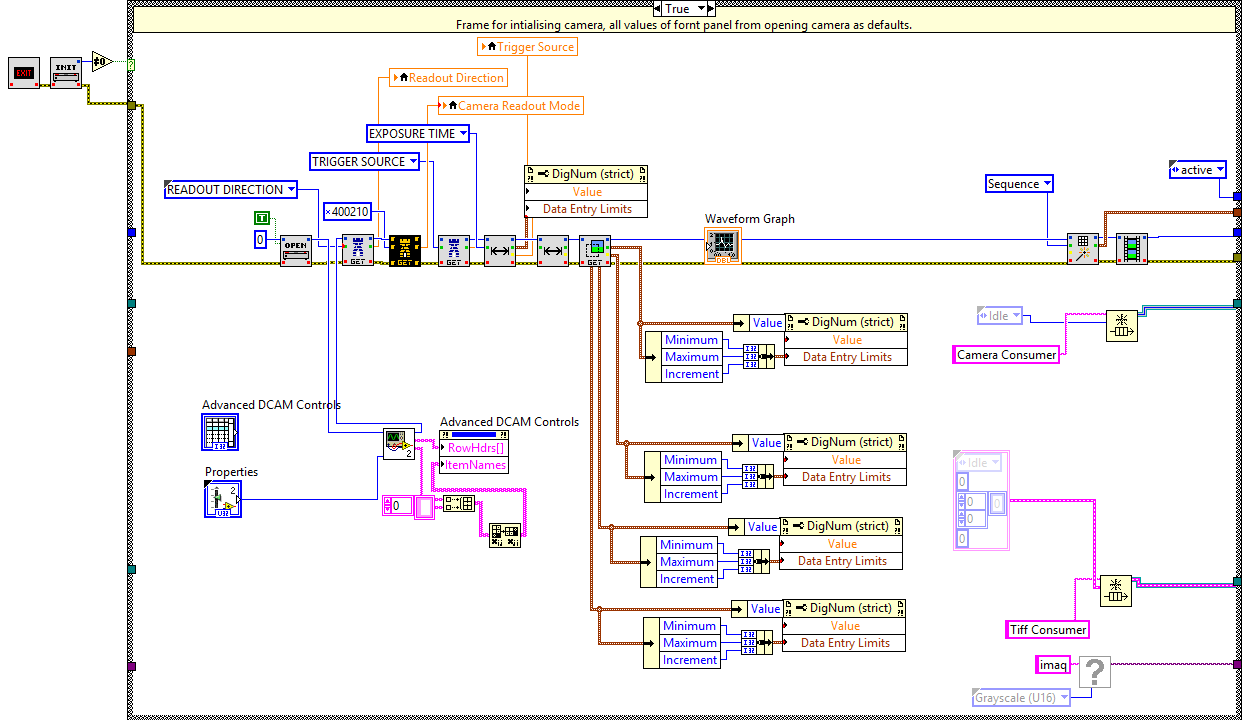
\includegraphics[width=\linewidth]{Figures/camera_init}
% 	\caption[Camera initialisation state]{Camera initialisation, standard settings to produce a default video output.}
% 	\label{fig:camera_init}
% \end{figure}
%
% % The first mode extracts camera data directly to a temporary file on the hard drive (a \SI{300}{\mega\byte\per\second}
% % solid state drive \SI{1}{\tera\byte}
% % raid, which is typically sufficiently quick for standard operations) in an proprietary format which is later decrypted by the slave loop in parallel to the camera loop producing the files.
% % Each temporary file contains a simple stack of images, designed such that each stack would be a full three dimensional scan of a volume.
% % To avoid overwriting, each temporary file was automatically named by a number with a six digit upper limit, far beyond the limitations of the hard drive capacity.
%
% \begin{figure}
% 	\centering
% 	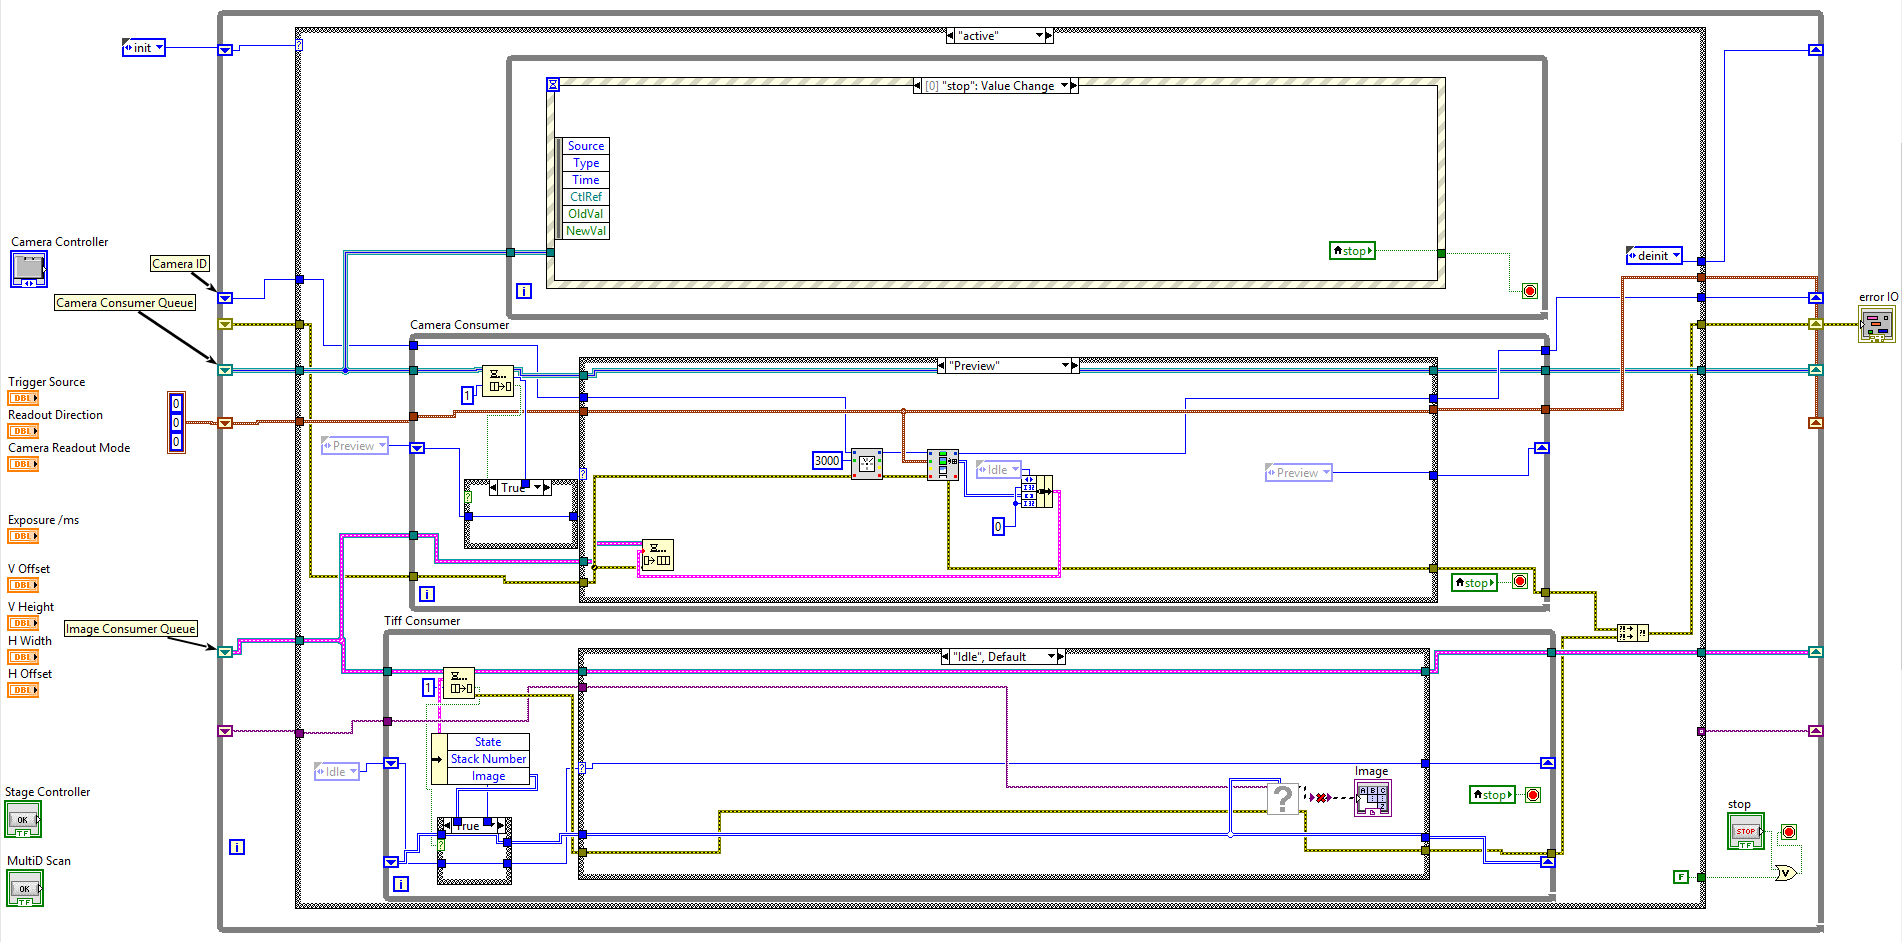
\includegraphics[width=\linewidth]{Figures/camera_active}
% 	\caption[Camera active state]{Camera active, a three stage consumer producer architecture which passes commands from top to bottom.
% The top loop sends user commands to the middle loop which controls the active status and frame collection, the bottom loop then saves and processes the image data produced in parallel.}
% 	\label{fig:camera_active}
% \end{figure}
%
% % The second mode records camera data directly to the computer's RAM which has much faster write speeds but is more limited in capacity to \SI{32}{\giga\byte}
% % in the current machine.
% % \footnote{For the camera to interface with the older software which controls the waveform generation it needs to have the same LabVIEW environment.
% % Unfortunately the old code was written in \SI{32}{\bit}
% % LabVIEW with a Mathscript module that has no \SI{64}{\bit}
% %  option as of yet.
% % This means that the waveform generation software will need to be completely rewritten if the RAM writing record mode is ever fully needed; \SI{32}{\bit}
% % systems are limited to \SI{2}{\giga\byte}
% % RAM considering the camera can output \SI{600}{\mega\byte\per\second}
% % this would overfill very quickly.
% % That said, the record to harddrive function can run perfectly well in a \SI{32}{\bit}
% % environment.
% % Horses for courses.}
%
%
% % \paragraph{Virtual Slit}
% %
% % The \textit{Orca 4v2} has this slit scanning mode embedded in its firmware and is accessible from the supplied software.
% % Inducing this within LabVIEW requires sending values to specific hex addresses using \textit{advanced\_property} functions.
% % Two modes were implemented, a manual mode for debugging purposes, and an automated mode which reads the current input to create a suitably synchronised rolling shutter, see Figure \ref{fig:camera_virtual_slit_module}.
%
% \begin{figure}
% \centering
% 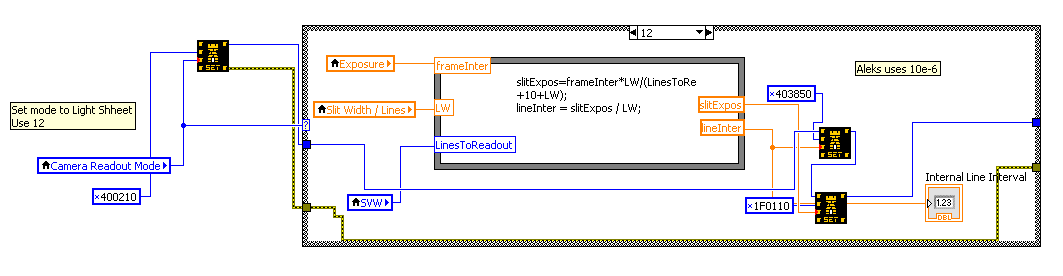
\includegraphics[width=0.7\linewidth]{Figures/camera_virtual_slit_module}
% \caption[LabVIEW virtual slit scanning module]{Module which prepares the sCMOS camera for virtual slit scanning.}
% \label{fig:camera_virtual_slit_module}
% \end{figure}
%
% %
% % \begin{figure}
% % \centering
% % 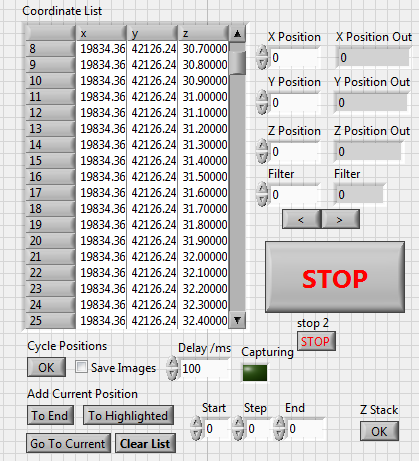
\includegraphics[]{Figures/xyz_front}
% % \caption[XYZ Controller front panel]{Front panel of the XYZ stage controller.
% % The arbitrary \SI{10} value in the mathmodule is a \SI{10}{\milli\second} delay inherent to the electronics of the camera.}
% % \label{fig:xyz_front}
% % \end{figure}
%
% % \subsubsection{Waveform module}
% %
% % %
% %
% % This module of the LabVIEW controller is the most crucial as it is the driver and synchronisation of the signals controller the scanning mirrors, focus stepper and tunable lens system if it is implemented.
% % This module will also serve as an advanced calibration routine for the microscope to control.
% %
% % \paragraph{Signal Train}~
% %
% % When creating the virtual light sheet the most intuitive signal to send would be a high frequency triangular waveform with a peak-to-peak voltage equal proportionate to the field of view of the image; however, as a mirror on a galvanometer scanner is a relativity large inertia mass, the peaks and troughs of the waveform would not only over shoot but also cause excessive stress and potentially break the scanner.
% % To circumvent this issue the mirror is returned to its base position sinusoidally, after each field of view scan, as the gradient of a sinusoid at its own peak is zero moving smoothly to zero again at its trough.
% %
% % It is unlikely that the virtual light sheet will be perfectly flat relative to detection, to this end the virtual light sheet can actually be twisted by synchronising the $z$ scanning mirror to the virtual sheet mirror tilting it by a gradient.
% % To create a full three dimensional scan the $z$ scanning mirror is offset along with its gradient step wise as seen in Figure \ref{fig:Signals}.
%
% \begin{figure}
% \centering
% 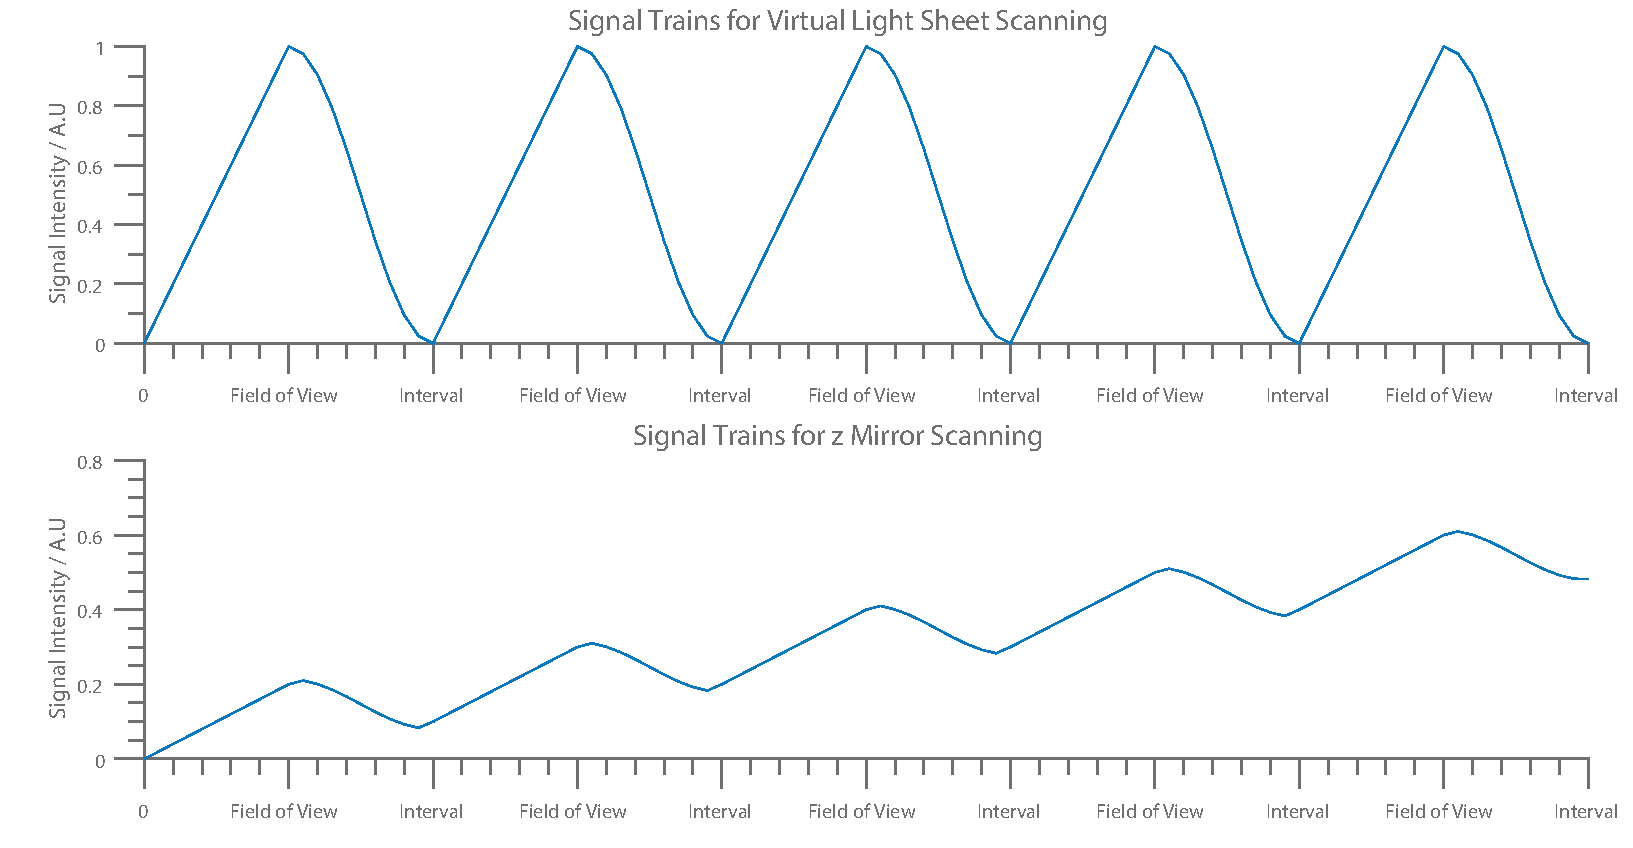
\includegraphics[width=\linewidth]{Figures/Signals}
% \caption[Light Sheet Signal Trains]{Signal Trains for Light Sheet and z axis mirror scanning.
% Each mirror scans and relaxes sinusoidally to avoid damage in the interval period.
% The z mirror components for a tilted light sheet using a slight gradient, this gradient is then applied to each Light Sheet scan before the z mirror is offset to scan a different volume of the sample.
% Intensities are in arbitrary units but are calibrated for within the real system}
% \label{fig:Signals}
% \end{figure}
%
%
% % \begin{table}
% %
% % 	\centering
% %
% % 	\begin{tabular}{lrrrrl}
% % 		\toprule Wavelength & \textcolor{455nm}{455} & \textcolor{488nm}{488} & \textcolor{561nm}{561} & \textcolor{647nm}{647} & \SI{\pm2}{\nano\meter} \\
% % 		\midrule
% % 		Output Power &  \num{100}&  \num{150}&  \num{150}&  \num{120}&  \SI{}{\milli\watt}\\
% % 		$M^2$ (Beam Quality) &  \num{<1.2} &  \num{<1.2}& \num{<1.1}& \num{<1.2}& \SI{}{\AU} \\
% % 		Beam Diameter &  \num{0.6}& \num{0.8}&  \num{0.7}& \num{0.9}& \SI{\pm 0.1}{\milli\meter}\\
% % 		Beam Divergence &  \num{<1.2}&  \num{<1.2}& \num{<1.2}&  \num{<1.3}&  \SI{}{\milli\radian} \\
% % 		Long-term Power Stability &  \num{<2}&  \num{<2}&  \num{<2}&  \num{<2}& \SI{}{\percent} (\SI{8}{\hour} \SI{\pm 3}{\celsius})\\
% % 		Laser Drive Modes & \multicolumn{5}{>{\centering\arraybackslash}p{8cm}}{\small{Continuous Wave, Analogue Modulation, Digital Modulation and Computer Control.}} \\
% % 		\bottomrule
% % 	\end{tabular}
% % 	\caption[Excitation lasers]{Significant information regarding the excitation laser emission sources.}
% % 	\label{table:laser}
% % \end{table}
%
% % \begin{figure}
% % \centering
% % 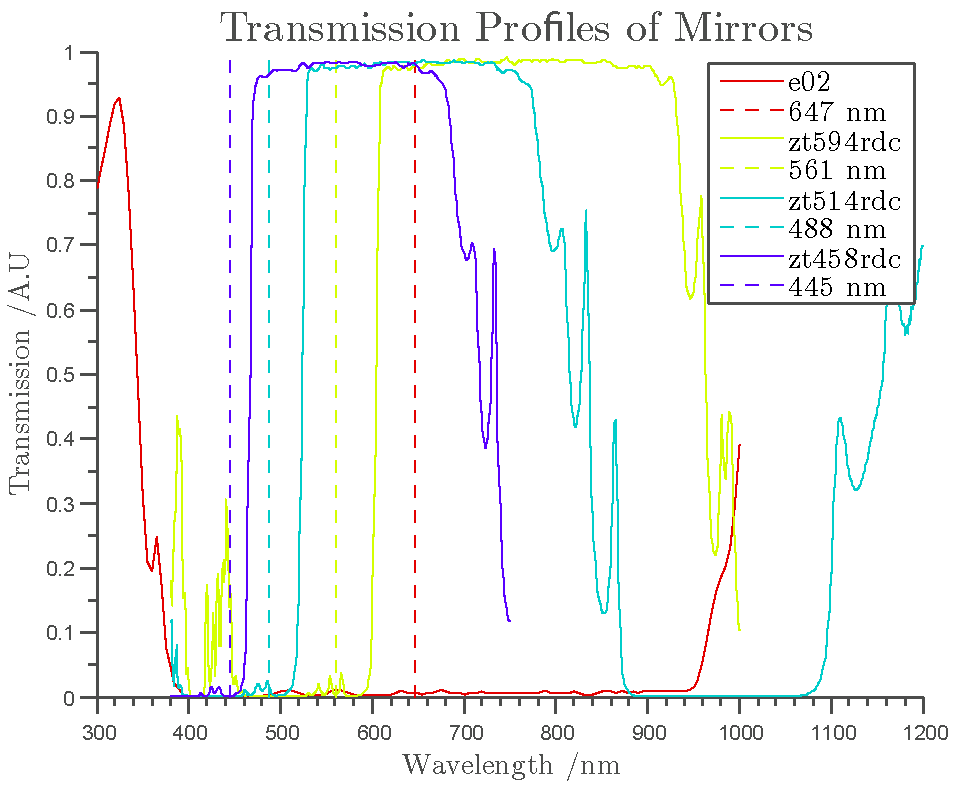
\includegraphics[width=0.7\linewidth]{Figures/Excitation}
% % \caption[Dichroic transmission profiles]{Transmission Profile for Dichroic mirrors used demonstrating that each mirror will reflect only the wavelength intended.}
% % \label{fig:Excitation}
% % \end{figure}
%
% % \subsubsection{Structured Illumination}
% %
% % An SLM can be used in two modalities, either it can be imaged onto the back aperture of the objective or conjugated.
% % When imaged onto the back aperture it directly manipulates Fourier space.
% % The primary use of the SLM in this system was to create Bessel beam illumination, with that in mind it was decided that the SLM should be imaged  onto the sample \cite{Fahrbach2010e}.
% % As Bessel beam needs only an annual ring in the Fourier domain, the majority of the light incident on the SLM would therefore be lost.
% % For this reason the SLM will be imaging onto the sample directly using a minimum focal length of \SI{47}{\centi\meter}, see Appendix \ref{appen:optdes} for details.
